\documentclass[a4paper,12pt, oneside]{book}

%\usepackage{fullpage}
\usepackage[italian]{babel}
\usepackage[utf8]{inputenc}
\usepackage{amssymb}
\usepackage{amsthm}
\usepackage{graphics}
\usepackage{amsfonts}
\usepackage{amsmath}
\usepackage{amstext}
\usepackage{engrec}
\usepackage{cancel}
\usepackage{rotating}
\usepackage[safe,extra]{tipa}
\usepackage{showkeys}
\usepackage{multirow}
\usepackage{hyperref}
\usepackage{microtype}
\usepackage{enumerate}
\usepackage{braket}
\usepackage{marginnote}
\usepackage{pgfplots}
\usepackage{cancel}
\usepackage{polynom}
\usepackage{booktabs}
\usepackage{enumitem}
\usepackage{framed}
\usepackage{pdfpages}
\usepackage{pgfplots}
\usepackage{fancyhdr}
\pagestyle{fancy}
\fancyhead[LE,RO]{\slshape \rightmark}
\fancyhead[LO,RE]{\slshape \leftmark}
\fancyfoot[C]{\thepage}



\title{Architettura degli Elaboratori}
\author{UniShare\\\\Davide Cozzi\\\href{https://t.me/dlcgold}{@dlcgold}\\}
\date{}

\pgfplotsset{compat=1.13}
\begin{document}
\maketitle

\definecolor{shadecolor}{gray}{0.80}

\newtheorem{teorema}{Teorema}
\newtheorem{definizione}{Definizione}
\newtheorem{esempio}{Esempio}
\newtheorem{corollario}{Corollario}
\newtheorem{lemma}{Lemma}
\newtheorem{osservazione}{Osservazione}
\newtheorem{nota}{Nota}
\newtheorem{esercizio}{Esercizio}
\tableofcontents
\renewcommand{\chaptermark}[1]{%
\markboth{\chaptername
\ \thechapter.\ #1}{}}
\renewcommand{\sectionmark}[1]{\markright{\thesection.\ #1}}
\chapter{Introduzione}
\textbf{Questi \textit{NON} sono appunti presi a lezione ma sono bensì un riassunto tratto da libro e slide del corso (la parte riguardante I/O deve essere ancora ultimata, attualmente sono presenti quasi unicamente suddette slide). Si assicura la probabile presenza di errori. Per eventuali proposte di correzione effettuare una pull request. Link: } \url{https://github.com/dlcgold/Appunti}.\\
\textbf{Grazie mille e buono studio!}
\chapter{Rappresentazione dell'informazione}
Innanzitutto si ha che quando si hanno $n$ bit si possono avere $2^n$ configurazioni diverse di bit. Quando dichiaro una variabile sto dichiarando una zona di memoria che contiene i bit di quel valore. Il numero di bit è finito.
\begin{nota}
Per indicare una base si usa la notazione $|_{base}$
\end{nota}
\begin{esempio}
$n=8$ comporta $256$ codici, quindi non permette la rappresentazioni di numeri negativi o maggiori di $255$. Si avranno quindi le seguenti rappresentazioni numeriche in 8 bit:
\begin{itemize}
\item $00000000=0\,|_{10}$
\item $00000001=1\,|_{10}$
\item $11111111=255\,|_{10}$
\end{itemize}
\end{esempio}
\begin{esempio}
Proviamo ora la conversione di numeri binari:\\
\textbf{da decimale a binario}:\\
converto $140|_{10}$ in binario:
$$\frac{140}{2}=70 \mbox{ con resto } 0$$
$$\frac{70}{2}=35 \mbox{ con resto } 0$$
$$\frac{35}{2}=17 \mbox{ con resto } 1$$
$$\frac{17}{2}=8 \mbox{ con resto } 1$$
$$\frac{8}{2}=4 \mbox{ con resto } 0$$
$$\frac{4}{2}=2 \mbox{ con resto } 0$$
$$\frac{2}{2}=1 \mbox{ con resto } 0$$
$$\frac{1}{2}=0 \mbox{ con resto } 1$$
quindi si ha: $10001100|_{2}$
\textbf{da binario a decimale}:\\
converto $10011|_{2}$ in decimali:
$$1\times 2^0=1\,+$$
$$1\times 2^1=2\,+$$
$$0\times 2^2=0\,+$$
$$0\times 2^3=0\,+$$
$$1\times 2^4=16\,=$$
$$\rule{100pt}{.4pt}$$
$$19|_{10}$$
\end{esempio}
Il binario si trova nei contenitori di bit e lì non ha rappresentazione da destra a sinistra bensì ha una rappresentazione data dall'hardware (dalle saldature).
Se prendo $n=8$ so che i valori che si possono rappresentare sono nel range $[0,255]$ e negli intervalli prima e dopo non ho modo di rappresentare nulla con 8 bit, si ha quindi un'\textit{eccezione}, in questo caso un'\textit{overflow}. Inoltre si possono avere problemi nel rappresentare numeri che sono risultato di operazioni aritmetiche (soprattutto la divisione). Si possono inoltre avere problemi causati dalla precedenza degli operatori
\subsubsection{Modulo e segno}
Per poter rappresentare i numeri negativi, utilizzando sempre 8 bit, si utilizza 1 bit per rappresentare il segno, cambiando così il range dei valori rappresentabili, che diventa:
$$[-(2^{n-1}-1),(2^{n-1}-1)]$$
Si ha però un problema: lo zero viene rappresentato da due codici:
\begin{itemize}
\item $0=\overbrace{0}^{segno}0000000$
\item $0=\overbrace{1}^{segno}0000000$
\end{itemize}
Per ovviare a questo problema sono nate 2 soluzioni:
\begin{enumerate}
\item \textbf{Complemento a 2}:\\
Questa codifica consente nel prendere il binario di un valore, complementarne i valori (il cosiddetto \textit{complemento a 1}) ovvero dove avevo $1$ scriverò $0$, e viceversa, e infine sommo $1$ al risultato, ottenendo così l'opposto del valore di partenza. Si ottiene così un nuovo range per i valori:
$$[-2^{n-1},2^{n-1}-1]=[-128,127]$$
Inoltre una tecnica di questo tipo, oltre a togliere il problema del doppio zero, permette all'hardware che sa far le somme di saper fare anche le differenze (senza aver quindi necessità di cambiare hardware)
\begin{esempio}
prendo $01101010$, ne faccio il \textit{complemento a 1} e ottengo $10010101$. Ora sommo 1:
$$10010101 \, +$$
$$00000001=$$
$$\rule{70pt}{.4pt}$$
$$10010110$$
\end{esempio}
\item \textbf{Eccesso}:\\
Si hanno i numeri da $256=11111111$ a $0=00000000$, le traslo verso il basso di $128$, ottenendo così: $127=11111111$ e $-128=00000000$, eliminando quindi il problema del doppio zero.
\end{enumerate}
Entrambe le tecniche portano a definire 0 come numero positivo.
\subsubsection{Rappresentazione Esadecimale}
I binari sono spesso espressi in esadecimali, ovvero in base $16$. Si ha quindi la notazione $|_{16}$. In questa notazione si usano $16$ simboli grafici: \textit{0,1,2,3,4,5,6,7,8,9,A,B,C,D,E,F}. Si ha per esempio $$11\,|_{10}=A\,|_{16} \,\, e \,\, 16\,|_{10}=10\,|_{16}=\overbrace{0x16}^{altra\,\, notazione\,\, per\,\, gli\,\, esadecimali}$$
\begin{esempio}
Proviamo ora la conversione di numeri esadecimali:\\
\textbf{da esadecimale a decimale}:\\
converto $2A1|_{16}$ in decimali:
$$1\times 16^0=1\,+$$
$$A\times 16^1=10\times 16 = 160\,+$$
$$2\times 16^2=2 \times 256=512\,=$$
$$\rule{140pt}{.4pt}$$
$$673|_{10}$$
\textbf{da decimale a esadecimale}:\\
converto $6574|_{10}$ in esadecimali:
$$\frac{6574}{16}=410 \mbox{ con resto } 14$$
$$\frac{410}{16}=25 \mbox{ con resto } 10$$
$$\frac{25}{16}=1 \mbox{ con resto } 9$$
$$\frac{1}{16}=0 \mbox{ con resto } 1$$
\textit{e mi fermo perché ho quoziente 1}\\
abbiamo quindi:\\
$$1\,\,9\,\,10\,\,14=19AE\,|_{16}$$
\end{esempio}
\subsubsection{Errori e Precisione}
La precisione dei numeri interi è 1. Ci sono numeri, come quelli appartenenti a $\mathbb{Q}$ e $\mathbb{R}$, che non sono rappresentabili dagli interi. Si cerca quindi un'approssimazione di quella cifra scegliendo il codice intero più vicino, e l'errore sarà la distanza tra il codice e il valore vero.
Per la rappresentazione dei numeri non interi si hanno due modi:
\begin{enumerate}
\item \textbf{Numeri in Virgola Fissa}:\\
Si ha quando conosco i codici vicino al valore che cerco e posso quindi suddividere l'intervallo tra i due codici in parti uguali. In termini pratici assegno $m$ bit prestabiliti alla parte decimale e i restanti alla parte intera. Per esempio dividendo l'intervallo per 1000 avrò la precisione di un millesimo, con un errore di approssimazione costante. Quindi dati $n$ bit ne uso uno per il segno, $m$ per la parte decimale e il restante per la parte intera. La parte decimale è decisa a priori e si rappresenta come un numero naturale ma con esponenti negativi della base.
\begin{esempio}
trasformo $101.01|_{2}$ in decimali:\\
$$101 \rightarrow 1\times 2^2+ 0\times 2^1+1 \times 2^0=5$$
$$01\rightarrow 0\times 2^{-1}+1\times 2^{-2}=0.25$$
quindi $101.01|_{2}\rightarrow 5.25|_{10}$
\end{esempio}
\begin{esempio}
trasformo $5.125|_{10}$ in binario:\\
$$\frac{5}{2}=2 \mbox{ con resto } 1$$
$$\frac{2}{2}=1 \mbox{ con resto } 0$$
$$\frac{1}{2}=0 \mbox{ con resto } 1$$
quindi $101$.\\ 
Passo alla parte decimale:\\
$$0.125\times 2 = 0.25 \mbox{ ovvero } 0 \mbox{ con resto } 0.25$$
$$0.25\times 2 = 0.5 \mbox{ ovvero } 0 \mbox{ con resto } 0.5$$
$$0.5\times 2 = 1 \mbox{ ovvero } 1 \mbox{ con resto } 0$$
Quindi $5.125|_{10}\rightarrow 101.001|_{2}$
\end{esempio}
Si possono avere rappresentazioni periodiche. Si possono rappresentare pochi numeri e spesso in maniera non completa, con uno spreco di memoria per rappresentare gli zeri. 
\item \textbf{Numeri in Virgola Mobile}:\\
Si ha quando non si conosce l'intervallo tra due codici, e quindi l'intervallo non può essere suddiviso in parti uguali. In termini di alto livello stiamo parlando di \textit{Float} e \textit{Double}. Con la notazione in virgola mobile si ha che la spaziatura dei vari intervalli cresce proporzionalmente. Si ha quindi un errore assoluto (modulo della differenza tra valore reale e valore trovato) crescente e non costante mentre l'errore relativo (rapporto tra errore assoluto e media delle misurazioni) è costante.\\
Un numero si dice \textit{normalizzato} se, in virgola mobile, non possiede zeri iniziali (esempio $1,1\times 10^{-9}$).\\
Per la rappresentazione si cerca un compromesso tra la \textbf{mantissa} (il valore compreso tra $0$ e $1$ che viene posto nel campo dopo la virgola) e l'\textbf{esponente}, aumentando la prima si aumenta l'accuratezza mentre aumentando il secondo si aumenta il range di numeri rappresentabili. Nel MIPS si ha la seguente rappresentazione:\\
\begin{center}
$1$ bit segno + $8$ bit esponente + $23$ bit mantissa 
\end{center}
ovvero: 
$$(-1)^S\times F\times 2^E$$
con $F$ contenuto del campo mantissa e $E$ contenuto del campo esponente. Nel MIPS si possono rappresentare numeri frazionari piccoli quanto $2|_{10}\times 10^{-38}$ e grandi $2|_{10}\times 10^{38}$, ma se l'esponete è troppo grande si finisce in \textit{overflow} come si può finire in \textit{underflow} se la parte frazionaria è troppo piccola. Questa appena spiegata è la rappresentazione in \textit{singola precisione}. Si può avere la rappresentazione in \textit{doppia precisione} che in MIPS richiede 2 parole, una con un bit per il segno, $11$ per l'esponente e $20$ per la mantissa mentre l'altra dedica $32$ bit alla mantissa. Si ottiene così una mantissa a $52$ bit con la possibilità di rappresentare numeri numeri frazionari piccoli quanto $2|_{10}\times 10^{-308}$ e grandi $2|_{10}\times 10^{308}$ .  Inoltre lo standard IEE 754 prevede una \textit{polarizzazione} pari a $127$ per la singola precisione in modo da ottenere l'esponente più negativo con $00...00$ e quello più positivo $11...11$. Si ha quindi che $-1$  è rappresentato da $-1+127|_{10}=126|_{10}=01111110|_2$ e $+1$ con $1+127|_{10}=128_{10}=10000000|_2$. Per la doppia precisione si usa un esponente di $1023$. Con la polarizzazione si ha:
$$(-1)^S\times(1+\, mantissa\,)\times 2^{\,esponente\,-\,polarizzazione} $$
così, in singola precisione, si va da $\pm 1,000...|_2\times 2^{-126}$ a $\pm 1,111...|_2\times 2^{+127}$
\begin{esempio}
Si mostra la rappresentazione binaria IEEE 754 di $-0,75|_{10}$:\\
$-0,75$ può essere scritto come: 
$$-\frac{3}{4}|_{10}=-\frac{3}{2^2}|_{10}$$
quindi sapendo che $3|_{10}=11_{2}$ ho:
$$-\frac{11|_2}{2^2|_{10}}=-0,11|_2$$
in notazione scientifica è $-0,11|_2\times 2^0$ e in notazione scientifica normalizzata $-1,1|_{2}\times 2^{-1}$.\\ Si ha quindi:
$$(-1)^1\times (1+0,1000....|_2)\times 2^{126-127}$$
con tanti 0 nella mantissa quanti i bit, nella doppia precisione si avrà la stessa cosa con più zeri e con $2^{1022-1023}$
\end{esempio}
\begin{esempio}
Trovo il decimale dal seguente numero in virgola mobile: $1100000010100....0$.\\ Il bit di segno è uguale a $1$, il campo esponente è $10000001=129|_{10}$ e il campo mantissa contiene $1\times 2^{-2}=0.25|_{10}$. Ora uso l'equazione:
$$(-1)^1\times (1+0,25)\times 2^{129-127}= -1\times 1.25\times 4=-5,0$$
\end{esempio}
\end{enumerate}
\subsection{Tipi di Dati}
Tutte le moderne CPU usano lo standard \textbf{IEEE754} che permette alla mantissa di essere di $24$ bit  in quanto si rende implicito il primo bit ($1$):
\begin{itemize}
\item Single (float) $\rightarrow$ 32 bit
\item Double (double) $\rightarrow$ 54 bit
\item Extended $\rightarrow$ 80 bit
\end{itemize}
Dati (di ogni tipo) e ed istruzioni sono solo configurazioni di bit
Un Single (32 bit), per esempio, è così scomposto (da sinistra verso destra):
\begin{itemize}
\item \textbf{msb} (\textit{most significant bit}) $\rightarrow$ 1 bit (0 per il segno positivo, 1 per il segno negativo)
\item \textbf{exp} (\textit{exponent}) $\rightarrow$ 8 bit
\item \textbf{frac} (\textit{fraction}) $\rightarrow$ 22 bit
\item \textbf{lsb} (\textit{least significant bit}) $\rightarrow$ 1 bit (ultima cifra della parte frazionaria, mi dice se il nuemro è pari o dispari)
\begin{center}
\begin{tabular}{c|c|c|c}
\multicolumn{4}{c}{32 bit}\\ \hline
msb&exp&frac&lsb\\ \hline
1 bit & 8 bit & 22 bit & 1 bit\\ \hline
segno & esponenziale & \multicolumn{2}{c}{parte decimale}\\ \hline
\end{tabular}
\end{center}
\end{itemize}
\begin{esempio}[???]
Posso effettuare la trasformazione:\\
$001101011100\times 2^0\rightarrow \cancel{00}\,1,\overbrace{1010111100}^{significand}\times 2^{1001}$
\end{esempio}
A seguito la tabella per la codifica \textbf{EEE754}
\begin{center}
\begin{tabular}{c|c|c|c|c}
\multicolumn{2}{c}{Single Precision} & \multicolumn{2}{c}{Double Precision} & Object Rapresented\\ \hline
Exponent&Fraction&Exponent&Fraction\\ \hline
0&0&0&0&0\\ \hline
0&Nonzero&0&Nonzero&$\pm$ denormalized number\\ \hline
1-254&Anything&1-2046&Anything&$\pm$ floating-point number\\ \hline
255&0&2047&0&$\pm$ infinity\\ \hline
255&Nonzero&2047&Nonzero&$\pm$ NaN (\textit{Not a Number})\\ \hline
\end{tabular}
\end{center}
\subsubsection{Forma Denormalizzata}
Posso sfruttare degli spostamenti per rappresentare ulteriori numeri limitando la precisione, aumentando l'errore relativo. Nell'esponente dei denormalizzati c'è una configurazione di zeri.
\subsection{Varie Rappresentazioni}
\subsubsection{Rappresentazione di Caratteri}
Si ha:
\begin{itemize}
\item \textbf{ASCII}, a 7 bit, quindi $2^7=128$ caratteri
\item \textbf{UNICODE}, a 16 bit, quindi $2^{16}=65536$ caratteri
\end{itemize}
\subsubsection{Rappresentazioni di Audio e Immagini}
\begin{itemize}
\item Il suono viene convertito in tensione/grandezze elettriche analogiche e convertito con il campionamento binario
\item L'immagine viene convertita come per il suono ma converte i vari colori, in una determinata posizione, in dati binari
\end{itemize}
\newpage
\section{Esercizi}

\begin{esercizio}
converto $1101101|_2$ in esadecimale:\\
prima converto in decimali:
$$1\times 2^6+ 1\times 2^5+ 0\times 2^4 +1 \times 2^3+ 1\times 2^2 +0\times 2^1+1\times 2^0=64+32+8+4+1=109|_{10}$$
ora converto $109|_{10}$ in esadecimali:
$$\frac{109}{16}=6 \mbox{ con resto di } 13$$
$$\frac{6}{16}=0 \mbox{ con resto di } 6$$
quindi $1101101|_2=6D|_{16}$ 
\end{esercizio}
\begin{esercizio}
converto $52|_{16}$ in binario:\\
innanzitutto lo converto in decimale:
$$2\times 16^0=2\,+$$
$$5\times 16^1= 80\,=$$
$$\rule{140pt}{.4pt}$$
$$82|_{10}$$
ora converto $82|_{10}$ in binario:
$$\frac{82}{2}=41 \mbox{ con resto } 0$$
$$\frac{41}{2}=20 \mbox{ con resto } 1$$
$$\frac{20}{2}=10 \mbox{ con resto } 0$$
$$\frac{10}{2}=5 \mbox{ con resto } 0$$
$$\frac{5}{2}=2 \mbox{ con resto } 1$$
$$\frac{2}{2}=1 \mbox{ con resto } 0$$
$$\frac{1}{2}=0 \mbox{ con resto } 1$$
quindi $52|_{16}=1010010|_2$
\end{esercizio}
\begin{esercizio}
converto $-20|_{10}$ in binario a 8 bit con il \textit{complemento a 2}:
$$\frac{20}{2}=10 \mbox{ con resto } 0$$
$$\frac{10}{2}=5 \mbox{ con resto } 0$$
$$\frac{5}{2}=2 \mbox{ con resto } 1$$
$$\frac{2}{2}=1 \mbox{ con resto } 0$$
$$\frac{1}{2}=0 \mbox{ con resto } 1$$
quindi $20|_{10}=10100|_2$, che in 8 bit è $00010100$. Ora procedo col \textit{complemento a 1} e ottengo $01011$, in 8 bit $11101011$. Infine sommo $1$:
$$11101011\,+$$
$$00000001\,=$$
$$\rule{100pt}{.4pt}$$
$$11101100$$
Se procediamo col metodo modulo e segno si ha che si parte da $10100$, si converte in 7 bit $0010100$ e si aggiunge il \textit{MSB} ( essendo negativo si mette $1$) ottenendo $10010100$
\end{esercizio}
\begin{esercizio}[???]
siano $01001$ e $10001$ prima una rappresentazione in \textit{modulo e segno} e poi in \textit{complemento a 2}. Definire nei due casi quale è maggiore.\\
Parto dal modulo e segno ( si vede che il primo è maggiore anche dal fatto che è positivo mentre l'altro è negativo):\\
$01001$ sarebbe $1001$ quindi $+1001|_2=+9|_{10}$
$10001$ sarebbe $0001$ quindi $-0001|_2=-1|_{10}$\\
quindi $01001$ è maggiore.\\
Passiamo al \textit{complemento a 2}:\\
$01001$ sarebbe $01001-1=01000$ a cui applico il \textit{complemento a 1} ottenendo $10111|_2$. Lo converto in decimale:\\
$$2^0+2^1+2^2+2^4=1+2+4+16=23|_{10}$$ quindi stiamo ragionando del numero $-23|_{10}$\\
$10001$ sarebbe $10001-1=10000$  cui applico il \textit{complemento a 1} ottenendo $01111|_2$. Lo converto in decimale:\\
$$2^0+2^1+2^2+2^3=1+2+4+8=15|_{10}$$ quindi stiamo ragionando del numero $-15|_{10}$.\\quindi $10001$ è maggiore.
\end{esercizio}
\begin{esercizio}
Sommo $0x789$ con $0x987$:\\
$9+7=16$ quindi $0$ col riporto di $1$
$8+8+1=17$ quindi $1$ col riporto di $1$
$7+9+1=17$ quindi $1$ col riporto di $1$
$1+0=1$
quindi:

$$789\,+$$
$$987\,=$$
$$\rule{60pt}{.4pt}$$
$$1110$$
\end{esercizio}
\begin{esercizio}
Rappresento $-20$ per eccesso $128$, ovvero, dato che voglio $128=n^{k-1}$ avrò k=8 bit:\\
$-20+128=108|_{10}=01101100|_2$
\end{esercizio}
\begin{esercizio}
sia $00011100|_2$, con eccesso $128$, trovo il decimale corrispondente:\\
$00011100=28|_{10}$ quindi so che $x+128=28$ quindi $x=-100$, che è il decimale corrispondente a $00011100|_2$
\end{esercizio}
\begin{esercizio}
Innanzitutto si riporta la tabella ascii:\\
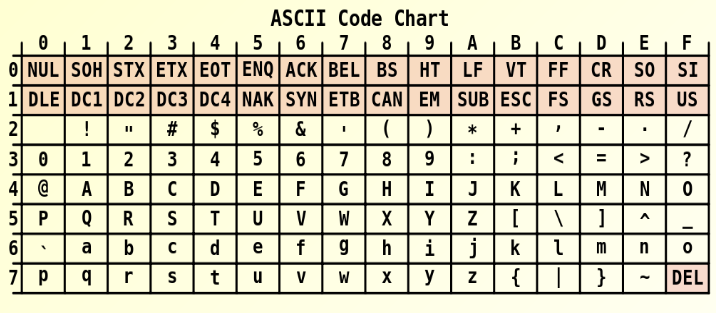
\includegraphics[scale=0.5]{img/ascii.png}
Converto la parola \textit{Bit} in decimale e esadecimale:\\
esadecimale = $42\,69\,74$\\
decimale = $ 066\,1051,116$
\end{esercizio}
\begin{esercizio}
Scrivo $13,25$ in virgola mobile:\\
trasformo $13$ in binario: $1101$.\\
Passo alla parte decimale:\\
$$0,25\times 2=0,5 \mbox{ ovvero } 0 \mbox{ col resto di } 0,5$$
$$0,5\times 2=1 \mbox{ ovvero } 1 \mbox{ col resto di } 0$$
quindi avrò $1101.01$ ovvero $1101.01\times 2^0=1.10101\times 2^3$. Si avrà:
$$(-1)^0\times (1+0,1010100...0)\times 2^{130-127}$$
e quindi la rappresentazione in virgola mobile su 32 bit  sarà:\\
segno positivo = $0$\\
esponente = $130$ = $10000010$\\
mantissa= $1010100000000000000000$\\
quindi:
$$13,25=0\,10000010\,1010100000000000000000$$
\end{esercizio}
\begin{esercizio}
Ricavo il decimale della seguente notazione in virgola mobile: $1\,10000000\,11000000000000000000000$:\\
segno negativo = $1$\\
esponente = $10000000|_2=128|_{10}$ quindi avrò $2^{128-127}=2$\\
parte frazionaria mantissa = $11000000000000000000000=0,75|_{10}$
quindi avrò: 
$$(-1)^{-1}\times (1+0,75)\times 2= -3,5$$
Quindi $1\,10000000\,11000000000000000000000=-3,5|_{10}$
\end{esercizio}

\chapter{Il computer}
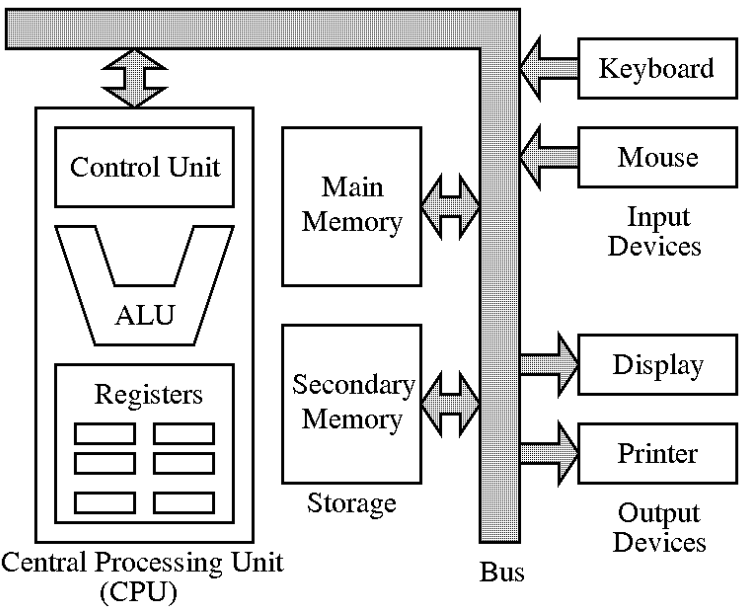
\includegraphics[scale=0.5]{img/computer.png}\\
Si introducono le componenti base di un calcolatore che permettono di realizzare le funzioni di input, output, elaborazione e memorizzazione dati:
\begin{itemize}
\item \textbf{Unità di Controllo:} è la componente del processore che invia i comandi all'unità di elaborazione dati, alla memoria e ai dispositivi di I/O secondo le istruzioni del programma
\item \textbf{Register File:} l'elemento che contiene i registri (\textit{R0...Rn}) che possono essere letti o scritti fornendo il numero del registro
\item \textbf{Memoria:} è dove vengono messi i programmi quando sono in esecuzione insieme ai dati da loro richiesti
\item \textbf{DRAM:} i chip di DRAM costituiscono la memoria, se ne possono quindi usare più di una per memorizzare le istruzioni di un programma. DRAM sta per \textit{memoria ad accesso casuale}. Si differenzia dalla normale memoria ad accesso sequenziale per il fatto che sono memorie il cui accesso richiede lo stesso tempo indipendentemente dalla particolare area di memoria
\item \textbf{Memoria Cache:} una memoria piccola ma veloce che agisce come "tampone", \textit{buffer}, nei confronti della DRAM. Essa è formata da SRAM,\textit{ memoria statica ad accesso casuale} 
\item \textbf{Memoria di Massa:} detta anche \textit{memoria secondaria} è una memoria non volatile dove si conservano i dati tra un'esecuzione e l'altra (HDD e SSD)
\item \textbf{Datapath:} detta anche \textit{unità di elaborazione dati, ALU} è la componente che esegue le operazioni logico-aritmetiche. Recupera i dati dai registri del processore, li processa nell'accumulatore e salva i risultati nel registro d'uscita
\item \textbf{Program Counter} è un registro del processore che conserva l'indirizzo di memoria della istruzione successiva. SI usa in un ciclo \textit{fetch-execute} che sarebbe una ripetizione infinita del caricamento di un'istruzione dal Program Couter, l'aggiornamento di quest'ultimo con l'istruzione successiva e l'esecuzione della stessa
\end{itemize}
\section{MIPS32}
Nell'architettura MIPS abbiamo tre tipi di istruzioni: \textit{R-Type, I-type e J-Type}. Andiamo ad analizzare il loro linguaggio macchina.
\newpage
\subsubsection{R-Type}
Solitamente rappresenta quelle operazioni che hanno due dati da elaborare e un risultato, per esempio \textit{add, sub, mul, div, and, or, ...}. Solitamente sono così formate:
$$6bit(op)+5bit(rs)+5bit(rt)+5bit(rd)+5bit(shamt)+6bit(funct)$$
Nel dettaglio si ha:
\begin{itemize}
\item \textbf{op:} \textit{operation code} identifica l'operazione, $000000$ è quello dell'R-Type
\item \textbf{registri:} \textit{rs} è il primo registro sorgente, \textit{rt} è il secondo registro sorgente e \textit{rd} è il registro destinazione
\item \textbf{Shamt:} \textit{shift amount} numero di posizioni di scorrimento, indica lo shift
\item \textbf{funct:} specifica la variante dell'operazione base
\end{itemize}
le istruzioni possono essere scritte in esadecimali. Per convertire in binario basta scrivere ogni singolo elemento del'esadecimale  in binario (se per esempio c'è \textit{e} avrò $1110$) e viceversa. Si ha la seguente tabella:\\
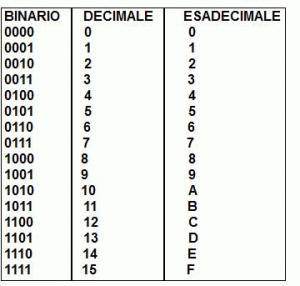
\includegraphics[scale=0.7]{img/conv.jpg}
\\Si aggiungono le tabelle coi registri e le operazioni base:
\newpage
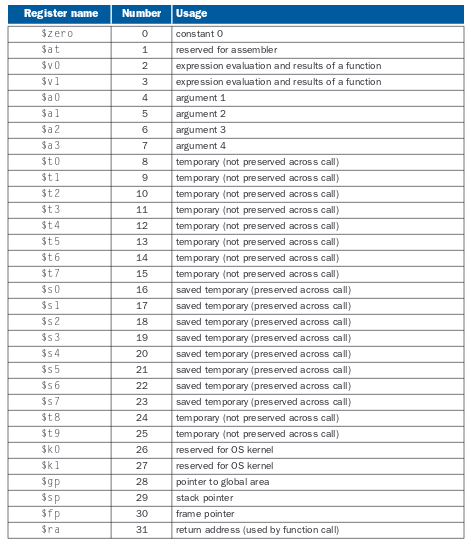
\includegraphics[scale=0.85]{img/reg.png}
\newpage
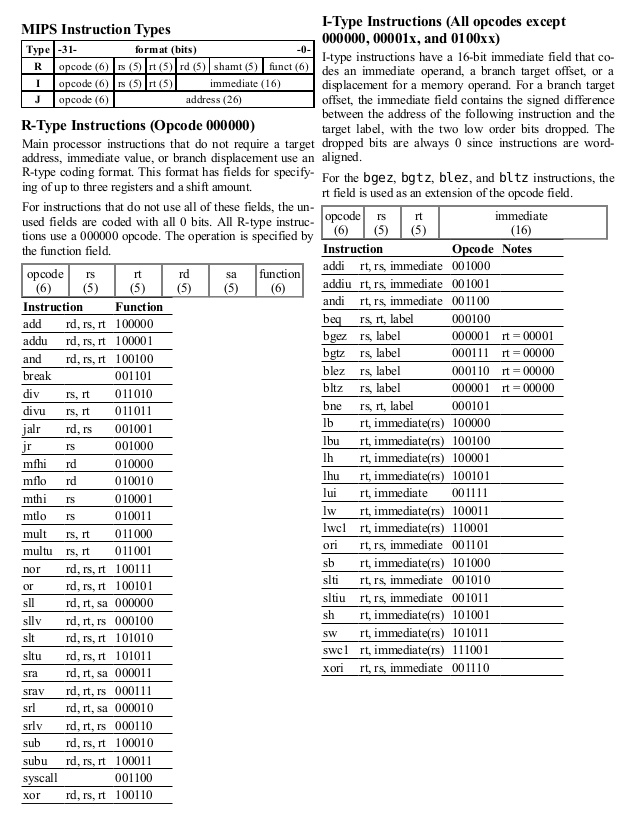
\includegraphics[scale=0.7]{img/r-i-code.jpg}
\newpage
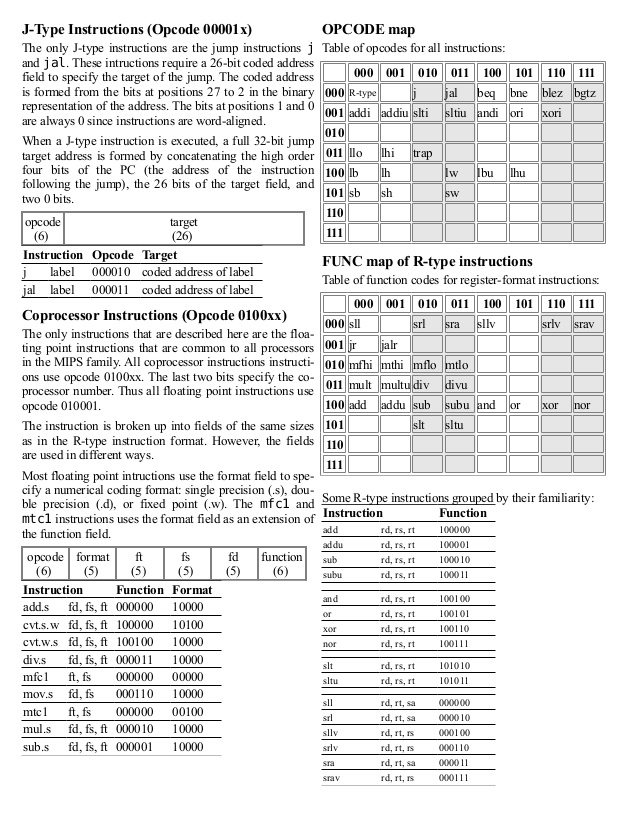
\includegraphics[scale=0.7]{img/j-code.jpg}
\newpage
per esempio:
$$000000\,01000\,01001\,01010\,00000\,100000$$
che in esadecimali è $0x01095020$ in quando possiamo notare come:\\ $0000\,0001\,0000\,1001\,0101\,0000\,0010\,0000$ sia facilmente convertibile con la tabella sopra. Si riconoscono:
\begin{itemize}
\item $op=000000$ quindi si ha un R-type
\item $rs=01000$ che è $8|_{10}$ e quindi il registro $\$t0$ è il primo registro sorgente
\item $rt=01001$ che è $9|_{10}$ e quindi il registro $\$t1$ è il secondo registro sorgente
\item $rd=01010$ che è $10|_{10}$ e quindi il registro $\$t2$ è il registro destinazione
\item $shamt=00000$
\item $funct=100000$ che è $32|_{10}$ e indica l'operazione \textit{add}
\end{itemize}
quindi avremo:
\begin{verbatim}
add $t0, $t1, $t2
\end{verbatim}
\subsubsection{I-type}
Si usa per eseguire operazioni con un dato contenuto in un registro e un numero costante (detto \textit{valore immediato}). Si hanno operazioni come \textit{addi, lw, sw, ...}. Solitamente sono così formate:
$$6bit(op)+5bit(rs)+5bit(rt)+16bit(imm)$$
Nel dettaglio si ha:
\begin{itemize}
\item \textbf{op:} \textit{operation code} identifica l'operazione, come faceva \textit{funct} per l'R-Type. Può quindi usare tutti gli opcode tranne $000000$, $000010$ e $000011$
\item \textbf{registri:} \textit{rs} è il registro sorgente e \textit{rt} è il registro destinazione.
\item \textbf{imm:} identifica un valore immediato o un offset (immediato)
\end{itemize}
Per esempio:
$$001000\,01000\,01010\,0000000000000100$$
ovvero:
\begin{itemize}
\item $op=001000$ che identifica \textit{addi}
\item $rs=01000$ che è $8|_{10}$ e quindi il registro $\$t0$ è il registro sorgente
\item $rt=01001$ che è $9|_{10}$ e quindi il registro $\$t1$ è il registro destinazione
\item $imm=0000000000000100$ identifica il valore $4$
\end{itemize}
quindi si avrà:
\begin{verbatim}
addi $t0, $t1, 4
\end{verbatim}
\subsubsection{J-Type}
Si usa per identificare i salti ed è molto semplice:
$$6bit(op)+26bit(address)$$
ovvero:
\begin{itemize}
\item \textbf{op:} \textit{operation code} $000010$ identifica \textit{j}, il salto \textit{incondizionato} e $000011$, il \textit{jal} che identifica il salto condizionato
\item \textbf{address:} \textit{rs} è il registro a cui saltare.
\end{itemize}
\chapter{Reti Sequenziali e Combinatorie}
Le parti principali di un computer sono costruite da circuiti digitali che elaborando segnali logici identificati da $0$ e $1$. Alla base dei circuiti si hanno le porte logiche:
\begin{itemize}
\item \textbf{Somma Logica OR:} se almeno una variabile di ingresso è $1$ la variabile di uscita sarà $1$\\
\\
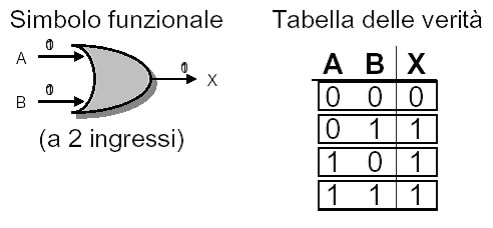
\includegraphics[scale=0.5]{img/or.jpg}
\item \textbf{Prodotto Logico AND:} la variabile di uscita è $1$ sse entrambe quelle di ingresso sono $1$:\\
\\
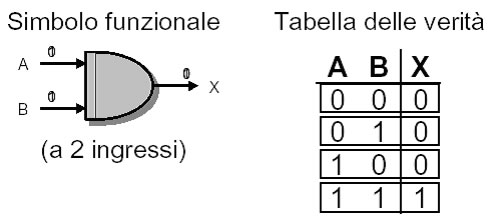
\includegraphics[scale=0.5]{img/and.jpg}
\item \textbf{Negazione NOT:} l'uscita sarà la variabile opposta a quella d'ingresso:\\
\\
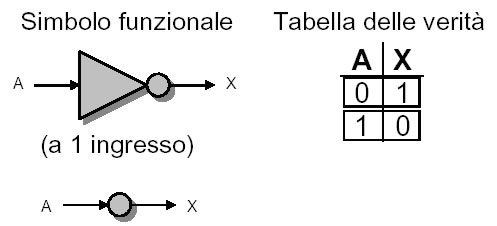
\includegraphics[scale=0.5]{img/not.jpg}\\
Essa può essere aggiunta alle porte OR e AND ottenendo NOR e NAND che avranno le uscite opposte a OR e AND. Per il NOR si ha che se almeno una variabile di ingresso è $1$ la variabile di uscita sarà $0$ e per il NAND che la variabile di uscita è $0$ sse entrambe quelle di ingresso sono $1$ (usando solo la porta NAND si possono ottenere le porte AND, OR e NOT, si chiama \textit{universalità di NAND}). Si ha inoltre la porta XOR (\textit{OR esclusivo}) che ha come uscita $1$ sse le variabili d'ingresso sono diverse:\\
\\
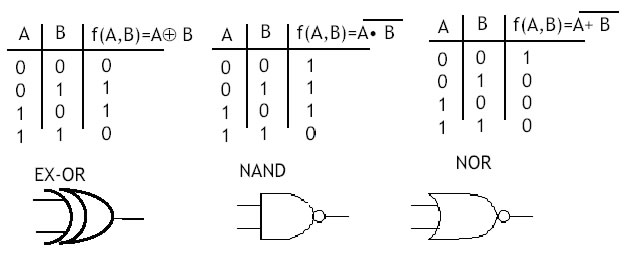
\includegraphics[scale=0.57]{img/nornand.jpg}\\
\end{itemize}
Collegando queste porte posso ottenere tutti i circuiti digitali. Si possono ottenere:
\begin{itemize}
\item \textbf{Circuiti Combinatori} dove le uscite dipendono unicamente dalle entrate
\item \textbf{Circuiti Sequenziali} dove le uscite dipendono anche dallo stato interno del circuito
\end{itemize}
\newpage
Vediamo alcuni circuiti logici famosi:
\begin{itemize}
\item \textbf{Decoder:} il più comune decoder prende in ingresso \textit{n} bit e ha $2^n$ uscite dove però viene presa una sola uscita data dalla combinazione delle entrate. Il decoder traduce il segnale d'ingresso su $n$ bit in un segnale che corrisponde al binario dell'ingresso. Gli output sono nominati \textit{out0,...,out 2n-1}. Se il valore in ingresso è \textit{x} si avrà true sull'uscita \textit{out x} e false su tutte le altre. Esiste anche l'\textbf{Encoder}, che prende in ingresso $2^n$ bit e ne ha $n$ in uscita. Ecco un esempio con $3$ bit in ingresso, e quindi $2^3=8$ bit in uscita:
\begin{center}
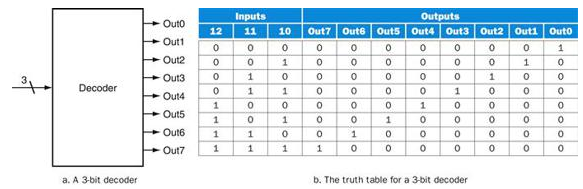
\includegraphics[scale=0.65]{img/dec.png}\\
\end{center}
Si nota che se per esempio di ha in ingresso $101|_2=5|_{10}$ si avrà $1$, ovvero true, solamente su \textit{out5}
\item \textbf{Multiplexor o Multiplexer:} si ha un'uscita uguale ad uno degli ingressi, scelto mediante un segnale di controllo. Si può usare un numero arbitrario di dati in ingresso, se ci sono due ingressi si ha un solo segnale di controllo, se se ne hanno $n$ si hanno $log_2(n)$ segnali di controllo. Ecco un esempio di un Multiplexor a due ingressi (\textit{A} e \textit{B}), con il segnale di controllo \textit{S}, che rappresenta la seguente operazione, di uscita $C$:
$$C=(A\cdot S)+(B\cdot S)$$ 
\begin{center}
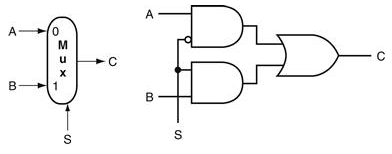
\includegraphics[scale=0.65]{img/mult.png}\\
\end{center}
se fosse stato formato da $n$ input si avrebbe avuto la seguente composizione:
\begin{enumerate}
\item un decoder che genera $n$ segnali, ciascuno corrispondente ad un diverso valore dell'ingresso di selezione 
\item una serie di $n$ porte AND ciascuna che combina uno degli input con un segnale dal decoder
\item una singola porta OR che raccoglie le uscite delle porte AND
\end{enumerate}
\item \textbf{Two-Level-logic e PLA (Programmable Logic Arrays:} si è visto che ogni funzione logica si può rappresentare con le porte OR, AND e NOT . Si può avere la TWO-Level-Rappresentation usando appunto unicamente le porte AND e OR, con al più un NOT finale. Per l'equazione 
$$E=((A\cdot B)+(A\cdot C)+(B\cdot C))\cdot (\overline{A\cdot B\cdot C)}$$
si ha:
\begin{enumerate}
\item \textbf{Somma di Prodotti:} è la rappresentazione della somma logica (OR) mediante i prodotti logici (AND):
$$E=(A\cdot B\cdot \overline{C})+(A\cdot C\cdot \overline{B})+(B\cdot C\cdot \overline{A})$$
\item \textbf{Prodotto di Somme:} è l'esatto opposto della Somma di prodotti:
$$E=(\overline{(\overline{A}+\overline{B}+C)\cdot (\overline{A}+\overline{C}+B)\cdot (\overline{B}+\overline{C}+A) })$$
\end{enumerate}
\newpage
Si userà soprattutto la \textit{Somma di Prodotti} che viene rappresentata dalla PLA. Una PLA ha un insieme di inputs e i relativi complementi (ottenuti grazie a degli invertitori) e due stadi di logica. Il primo stadio è un array di porte AND che formano un insieme di \textit{termini prodotto} (detti \textit{ninterms}), ciascuno dei quali può consistere in uno qualsiasi degli input o dei loro complementi. Il secondo stadio è un array di porte OR ciascuna delle quali effettua una somma logica di un certo numero di \textit{termini prodotto}. Ecco una rappresentazione schematica:\\
\begin{center}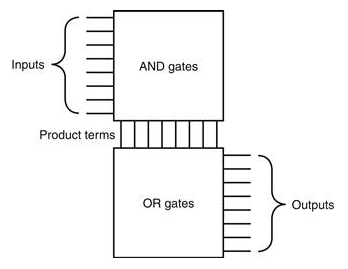
\includegraphics[scale=0.65]{img/pla.png}\end{center}
Una PLA può implementare direttamente la tavola di verità di una certa funzione logica, con molteplici input e output. Dato che ogni ingresso per il quale l'output è true richiede un \textit{termine prodotto} ci sarà una riga corrispondente nella PLA. Ogni output corrisponde ad una certa riga di porte OR nel secondo stadio. La grandezza della PLA è data dalla somma delle lunghezze dei due array di porte AND e OR (dette \textit{AND plane} e \textit{OR plane}. La \textit{AND plane} sarà pari a $numero\,\, input\,\, \times \,\, numero\,\, ninterms\,\, differenti$ mentre la \textit{OR plane} sarà pari a $numero\,\, output\,\, \times \,\, numero\,\, ninterms\,\, differenti$. Nella PLA solo la tavola di verità che produce true ha delle porte logiche associate e esiste un solo ingresso per ogni minterm differente (due \textit{termini prodotto} uguali non hanno due ingressi diversi).
\newpage
 Vediamo un espio dove si hanno A,B,C come input la cui tabella rappresenta lo stadio AND) e D,E,F come output la cui tabella rappresenta lo stadio OR). Ecco la tavola di verità:\\
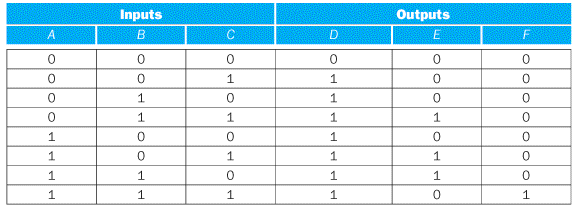
\includegraphics[scale=0.58]{img/pla1.png}\\
che può essere rappresentata con le porte logiche (l'ingresso $A=0,\,B=0,\,C=0$ non è presente perché non da output):\\
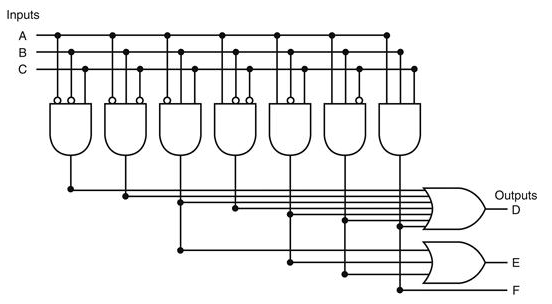
\includegraphics[scale=0.58]{img/pla2.png}\\
o mediante uno schema dove i pallini scuri sono gli $1$ e si ha una rappresentazione mediante linee verticali e orizzontali:
\begin{center}
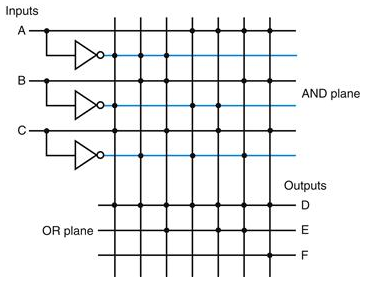
\includegraphics[scale=0.565]{img/pla3.png}\end{center}
\newpage
\item \textbf{ROM (Read Only Memory):} una ROM è detta memoria in quanto è un'insieme di locazioni che possono essere lette, tuttavia il contenuto è fisso e deciso nel momento della produzione. Esistono poi le PROM, ovvero le ROM \textit{programmable} che possono essere programmate elettronicamente dopo il momento della produzione. Infine esistono le EPROM, ovvero le PROM \textit{eresable}, che possono essere riscritte, cancellando con la luce ultravioletta il contenuto precedente. Sono quindi memorie di sola lettura (tranne durante la produzione e la fase di debug). Una ROM è formata da un insieme di funzioni logiche che forniscono gli indirizzi di ingresso e le uscite. Il numero di bit presenti in ciascun elemento indirizzabile  determina il numero di bit d'uscita ed è detto \textit{ampiezza} della ROM, per $n$ linee di input si ha un'ampiezza pari a $n$. Se la ROM contiene $2^n$ elementi indirizzabili (detta \textit{altezza} della ROM) si hanno $n$ linee di input. Altezza e larghezza definiscono lo \textit{shape (forma)} dell ROM. Una ROM può codificare una collezione di funzioni logiche direttamente dalla tabella di verità, per esempio con $m$ funzioni e $n$ input ci serve una ROM con $n$ linee di indirizzo e $2n$ ingressi, con ogni ingresso largo $m$ bit. Gli ingressi nella tavola di verità sono gli ingressi nella ROM, mentre le uscite della tavola sono il contenuto della ROM. Se la tabella di verità è organizzata in modo tale che le entrate sono una sequenza di binari allora l'output farà si che il contenuto della ROM avrà lo stesso ordine. A differenza della PLA la ROM è totalmente codificata e quindi ha più entrate (che crescono in maniera esponenziale) e più termini prodotto (che crescono in numero più lentamente). Le ROM possono implementare qualsiasi funzione logica abbinando input e output. Diventa così semplice cambiare il contenuto della ROM se cambia la funzione logica, dato che la grandezza della ROM non cambia
\end{itemize}
\newpage
Si elencano ora altri aspetti, strutture o circuiti:
\begin{itemize}
%don't cares
\item \textbf{Bus:} è una collezione di linee di informazione unite da un singolo segnale logico. Per esempio nelle istruzioni MIPS il risultato di un'istruzione può essere scritto in un registro provenendo da una di due sorgenti. Un multiplexor sceglie quale dei due Bus (ciascuno largo 32bit) sarà scritto nel registro del risultato. Ovviamente il multiplexor a 1bit visto sopra dovrà essere replicato 32 volte. Nei disegni si rappresenta una linea diagonale sopra quella dell'input per rappresentare il numero di strutture (numero da indicare a fianco) necessarie, come in figura:\\
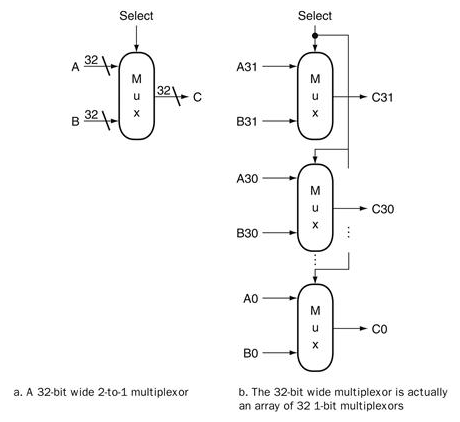
\includegraphics[scale=0.58]{img/mult2.png}\\
\item \textbf{Carry In e Carry Out:} il carry In rappresenta il riporto dell'operazione aritmetica precedente, il Carry Out rappresenta il riporto dell'operazione appena eseguita e diventa il Carry In di quell seguente
\item \textbf{Segnale di Clock:} nella logica sequenziale i segnali di clock sono necessari per determinare quando devono essere aggiornati gli elementi. Si ha quindi un segnale che evolve indipendentemente nel tempo con un certo periodo $T$ costante. Si ha la frequenza di clock data da $\nu=\frac{1}{T}$. Il ciclo di clock si divide in 2 parti, quando il clock è alto e quando è basso, tra basso e alto si ha il \textit{fronte (edge) di salita} e tra l'alto e il basso si ha il \textit{fronte (edge) di discesa}. Tutti i cambi di stato avvengono in corrispondenza di un fronte. \\Ecco una figura che semplifica quanto detto:\\
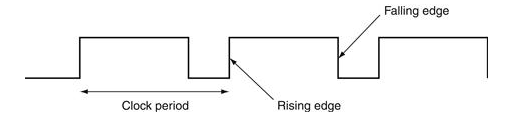
\includegraphics[scale=0.565]{img/clock.png}\\
\item \textbf{SR Latch:} è uno degli elementi di memoria più semplici, detto anche \textit{Set and Reset Latch}, è costituito da una coppia di porte NOR e il bit immagazzinato è portato all'output $Q$ e al suo complementare $\overline{Q}$. Se R e S non sono assegnate la coppia incrociata di coppie NOR agisce come un invertitore e salva i valori precedenti di $Q$ e $\overline{Q}$. Ecco un'immagine dell'SR Latch:
\begin{center}
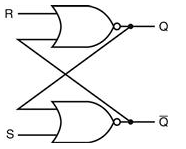
\includegraphics[scale=0.7]{img/srlatch.png}
\end{center}
Si ha il seguente schema:
\begin{center}
\begin{tabular}{|c|c|c|}
\hline
S & R & funzione\\
\hline
\hline
0 & 0 & Latch (memorizzazione)\\
\hline
0 & 1 & Reset: $Q=0$ e $\overline{Q}=1$\\
\hline
1 & 0 & Set: $Q=1$ e $\overline{Q}=0$\\
\hline
1 & 1 &  Errore, operazione non consentita\\
\hline
\end{tabular}
\end{center}
\item \textbf{D Latch:} ha 2 input e 2 output, dove gli input sono il valore da memorizzare, chiamato D, e il segnale di clock, chiamato C, che indica quando il latch deve leggere il valore sull'ingresso D e memorizzarlo. Gli output sono semplicemente il valore dello stato interno $Q$ e il suo complemento $\overline{Q}$. Quando il valore di clock C è affermato ($1$) si ha che il Latch è \textit{aperto} e il valore di $Q$ diventa il valore di D. Quando il clock non è affermato ($0$) si dice che il Latch è \textit{chiuso} e il valore di $Q$ è rimane lo stesso dell'ultima volta che il Latch è stato \textit{aperto}. Dato che $Q$ varia ogni volta che varia D questa struttura è anche detta \textit{Latch trasparente}.\\ \\ \\ \\Ecco un'immagine che rappresenta il D Latch:
\begin{center}
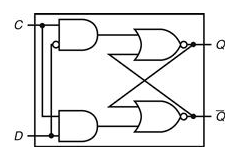
\includegraphics[scale=0.7]{img/dlatch.png}
\end{center}
ed ecco cosa succede schematicamente a D e $Q$ in corrispondenza del periodo di clock:
\begin{center}
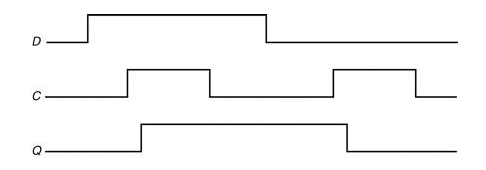
\includegraphics[scale=0.7]{img/dlatch2.png}
\textit{D assume un valore, quando si ha il fronte di C lo "scrive" in $Q$, poi assume un altro valore che viene scritto non appena si ha un altro fronte di C. Il tempo minimo per cui l'ingresso D deve rimanere valido prima del fronte di clock è detto \textbf{tempo di set-up (tempo di preparazione)} mentre il tempo minimo per cui deve rimanere valido dopo il fronte è detto \textbf{tempo di hold (tempo di mantenimento), che solitamente è circa 0. Fallimenti di questi tempi minimi possono comportare output non prevedibili}. Il valore salvato e l'output $Q$ cambiano entrambi quando C è alto}
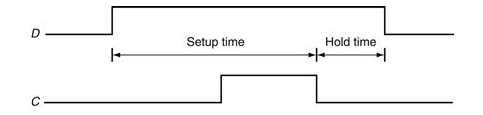
\includegraphics[scale=0.7]{img/time.png}
\end{center}
\newpage
\item \textbf{D Flip-Flop} si ha che un Flip-Flop è un elemento di memoria dove l'output è uguale al valore dello stato dentro l'elemento e si ha che lo stato cambia solo in un fronte di clock, può essere costruito in modo che l'azione venga svolta sia nel fronte di salita che in quello di discesa del clock ( o uno o l'altro). I Flip-Flop non sono \textit{trasparenti}, l'output cambia solo su un fronte di clock. Un D Flip-Flop è un Flip-Flop con una solo input di informazioni che salva il valore del segnale in input quando si ha un fronte di clock. 

Ecco un'immagine del D Flip-Flop che agisce nel fronte di discesa costruito da una coppia di D Latch:
\begin{center}
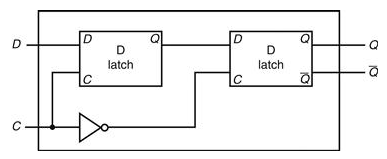
\includegraphics[scale=0.7]{img/dff.png}\\
\textit{Il primo Latch, chiamato \textbf{master}, e aperto quindi segue il valore di D solo se C è affermato. Quando il clock cade si chiude il primo Latch ma il secondo, chiamato \textbf{slave} è aperto e prende l'input dall'output del primo Latch}
\end{center}
ed ecco cosa succede schematicamente a D e $Q$ in corrispondenza del periodo di clock:
\begin{center}
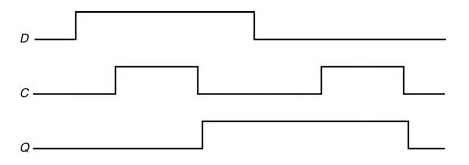
\includegraphics[scale=0.7]{img/dff2.png}\\
\textit{Quando C scende l'output di $Q$ salva il valore dell'input D}
\end{center}
\newpage
\item \textbf{Register File:} la struttura principale del nostro datapath è il Register File, che consiste da un insieme di registri che possono essere letti e scritti fornendo il numero del registro da utilizzare. Si può implementare con un decoder per ogni per ogni porta di lettura o scrittura e con una matrice di registri fatti da dei D Flip-Flop. Dato che leggere un registro non cambia  nessuno stato basta fornire in ingresso un indirizzo e si avrà come output l'informazione contenuta nel registro. Per scrivere un registro si avrà bisogno di 3 input:
\begin{enumerate}
\item il numero del registro
\item l'informazione da scrivere
\item un segnale di clock che controlli l'operazione di scrittura
\end{enumerate}
Le porte di lettura invece si possono implementare con 2 multiplexor \textit{n-to-1}, ciascuno di ampiezza pari al numero di bit presenti in ogni registro del Register File. 
\\A seguito un'immagine che rappresenta l'implementazione di 2 porte di lettura di registri per un Register File ampio 32 bit:
\begin{center}
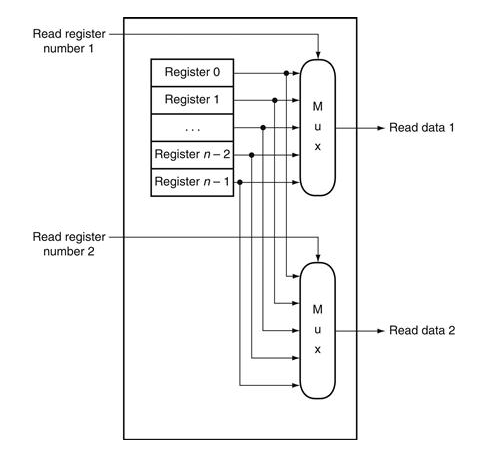
\includegraphics[scale=0.7]{img/reg2.png}
\end{center}
\newpage
\begin{center}
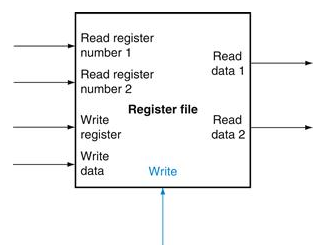
\includegraphics[scale=0.7]{img/reg1.png}\\
\textit{un Register File con due porte di lettura e una di scrittura ha 5 input e 2 output }
\end{center}
ecco invece l'implementazione di una porta di scrittura (un po' più complessa a causa del fatto che possiamo cambiare il contenuto solo del registro scelto). Per ottenerla si usa un decoder \textit{n-to-}$2^n$ che genera un segnale indicante il registro da usare. Tutti e tre gli input hanno \textit{setup time} e \textit{hold time} per consentire la corretta esecuzione dell'operazione:
\begin{center}
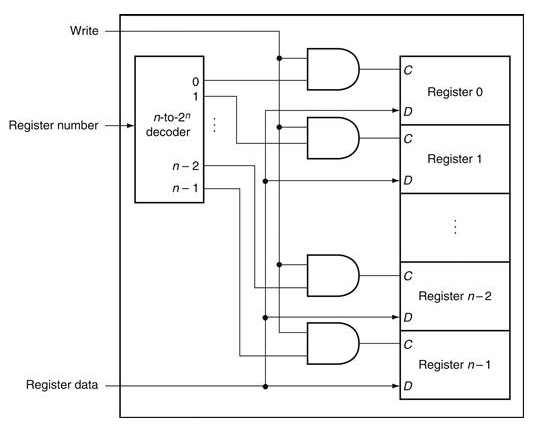
\includegraphics[scale=0.6]{img/reg3.png}
\end{center}
\newpage
Se lo stesso registro viene letto e scritto durante un ciclo di clock si ha che, dato che la scrittura avviene su un fronte del clock, il registro sarà valido durante la scrittura e il valore letto sarà quello scritto in un ciclo di clock precedente. Per leggere il valore in corso di scrittura servirebbero delle implementazioni aggiuntive alla logica del Register File. Si hanno i seguenti:
\begin{enumerate}
\item \textbf{Read Reg \#1:} numero del primo registro da leggere
\item \textbf{Read Reg \#2:} numero del secondo registro da leggere
\item \textbf{Read Data 1:} valore del primo registro letto sulla base del \textit{Read Reg \#1}
\item \textbf{Read Data 2:} valore del secondo registro letto sulla base del \textit{Read Reg \#2}
\item \textbf{Write Reg\#:} numero del registro su cui si deve scrivere
\item \textbf{Write Data: } valore del registro da scrivere in base a \textit{Write Reg\#}
\end{enumerate}
\item \textbf{SRAM (Static Random Access Memory):} è una memoria dove i dati sono salvati in maniera statica (come in un Flip-Flop). Più veloce della DRAM ma più costosa. Si hanno dei semplici circuiti integrati che sono gli array della memoria con solitamente una sola porta d'accesso, che provvede sia alla lettura che alla scrittura. Si ha un tempo di accesso fisso, anche se ci sono differenze tra lettura e scrittura. Si hanno inoltre configurazioni specifiche per il numero di locazioni indirizzabili e per l'ampiezza di ciascuno di essi. Per esempio una SRAM 4M$\times$8 provvede con 4M entrate, ciascuna di 8 bit, con quindi 22 linee di accesso (4M=$2^{22}$), un output a 8bit e un singolo dato in input da 8bit. Come nelle ROM si ha che il numero di locazioni indirizzabili è chiamato \textit{altezza} e il numero di bit per ciascuna unità è detto \textit{larghezza}. Vediamo lo schema di una SRAM 2M$\times$16, con i 21 indirizzi, i 16 dati in input, i 3 controlli e i 16 dati in output:
\begin{center}
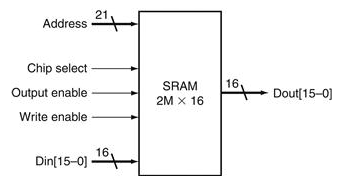
\includegraphics[scale=0.7]{img/sram.png}
\end{center}
\newpage
Per iniziare a leggere o scrivere il \textit{Chip Select}  deve essere attivo, per leggere bisogna anche attivare il segnale dell'output per indicare se il dato selezionato dall'indirizzo è attualmente guidato sui pin. L'attivare l'output è comodo per connettere più memorie verso un solo bus di output e per capire verso quale memoria indirizzare il bus. Il tempo di accesso in lettura è solitamente indicato dal ritardo (\textit{delay}) tra il tempo in cui l'output è abilitato e l'indirizzo è valido e il tempo che l'informazione si trova nell'output. I tempi di accesso variano tra i $0,5$ e i $2,4$ \textit{ns} per le parti più veloci e piccole (CMOS, \textit{complementary metal-oxide semiconductor}, si hanno tempi leggermente maggiori (tra i $2$ e i $12$ \textit{ns}) per le parti più grandi. Sono state prodotte anche SRAM a basso consumo, sia in stand-by che in uso, generalmente dalle $5$ alle $10$ volte più lente. Sono state sviluppate anche SRAM sincrone. Per scrivere servono il dato da scrivere e l'indirizzo. Quando sia il \textit{write enable} e il \textit{chip select} sono settati true il dato viene scritto nell'indirizzo specificato. Ovviamente si hanno i soliti \textit{setup time} e \textit{hold time}. Inoltre il \textit{write enable} non è controllato dal clock ma da un impulso \textit{pulse} con requisiti minimi di ampiezza. Il tempo totale della scrittura è dato dai due \textit{time} e da questo impulso. Grandi SRAM non possono essere costruite come il Register File a causa del $64$k-to-$1$ multiplexor necessario per una $64$K$\times$1 SRAM. Memorie più grandi usano quindi una linea di output condivisa, chiamata \textbf{bit line}. Per permettere a più sorgenti di veicolare  su una linea singola si usa un \textit{three-state buffer (detto anche tristate buffer)} che è dotato di due input (un segnale con l'informazione e un \textit{output enable}) e un singolo output (uno tra: \textit{asserted}, \textit{deasserted} e \textit{high impendance}). L'output del \textit{tristate buffer} è uguale all'input del segnale con l'informazione, o \textit{asserted} o \textit{deasserted}, se l'\textit{output enable} è \textit{asserted}, ed è altrimenti in uno stato di \textit{high impendance} che permette ad un altro \textit{tristate buffer}, con \textit{output enable} \textit{asserted}, di determinare il valore dell'output condiviso. I \textit{tristate buffer} sono incorporati nei Flip-Flop che formano le celle base della SRAM. 
\newpage
Ecco una un gruppo di 3 \textit{tristate buffer} che formano un multiplexor con un decoder come input:
\begin{center}
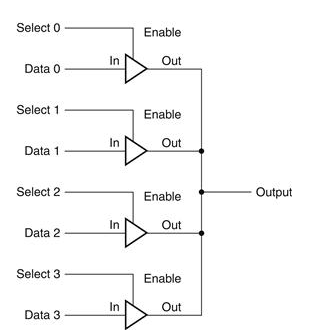
\includegraphics[scale=0.7]{img/sram2.png}
\end{center}
\newpage	
ed ecco una piccola SRAM 4$\times$2, costruita con un D Latch con un input chiamato \textit{enable} che controlla il \textit{three state} output:
\begin{center}
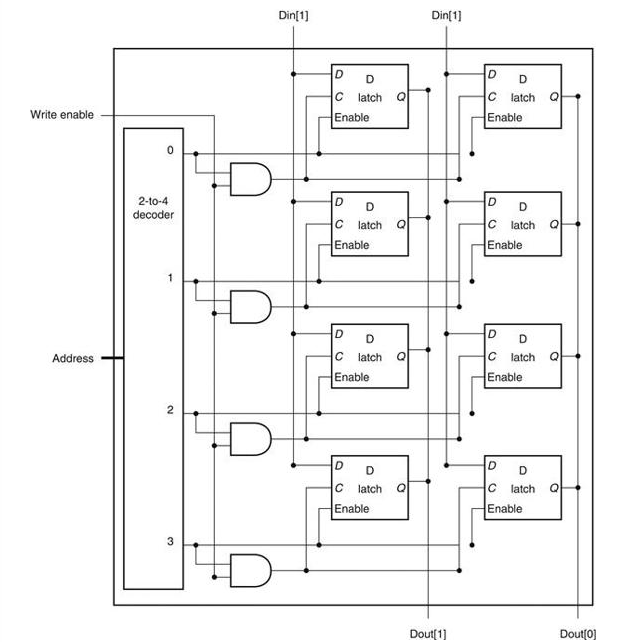
\includegraphics[scale=0.7]{img/sram3.png}
\textit{solo uno dei 4 input può essere asserito. Il decoder seleziona le celle da attivare, che a loro volta usano un \textit{three state output} connesso alla linea verticale che fornisce l'informazione richiesta. L'indirizzo che seleziona la cella è mandato ad uno degli insiemi di linee orizzontali dette \textit{word lines}. Si elimina l'uso di enormi multiplexor ma si ha ancora necessità di un grande decoder (per una 4m$\times$8 serve un decoder 22-to-4M) e tante word lines. per ovviare a questo problema le grandi memorie vengono organizzate in un array di rettangoli come nell'esempio seguente:}
\begin{center}
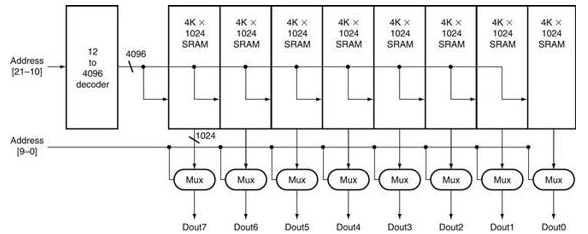
\includegraphics[scale=0.7]{img/sram4.png}
\end{center}
\end{center}
\item \textbf{DRAM (Dynamic Random Access Memory):} in queste memorie il dato è salvato come una carica in un condensatore. Un singolo transistor è usato per accedere a questa carica salvata, sia per leggere che per sovrascrivere. Queste memorie sono più economiche (la SRAM richiede da 4 a 6 transistor per bit, la DRAM 1). A causa del fatto che salva la carica in un condensatore la DRAM deve essere periodicamente \textit{refreshata} ed è per questo che è definita memoria \textit{dinamica}. Per il refresh bisogna leggere il dato e riscriverlo, comunque la carica si mantiene per molti millisecondi, quindi per milioni di cicli di clock (sono in uso ora anche DRAM che refreshano senza basarsi sul clock del processore). Per permettere l'accesso nonostante i continui refresh la DRAM usa una struttura di decodifica a due livelli che permette di refreshare un'intera riga (\textit{word line}) con un ciclo di lettura subito seguito da un ciclo di scrittura, occupando l'1\%, massimo il 2\%, dei cicli della DRAM, lasciando tutti gli altri per la lettura e la scrittura dei dati.\\
Il transistor dentro la cella è uno \textit{switch}, chiamato \textit{pass transistor}, come quello in figura:
\begin{center}
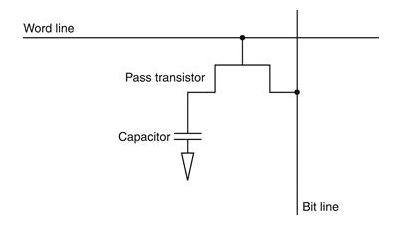
\includegraphics[scale=0.7]{img/dram.png}
\end{center}
quando il segnale sulla \textit{word line} è \textit{asserted} lo switch è chiuso, connettendo il condensatore alla \textit{bit line}. Nel caso della scrittura si ha che il valore da scrivere si mette nella \textit{bit line}, se è $1$ il condensatore si carica, altrimenti si scarica. La lettura è invece più complessa in qaunto la DRAM deve leggere cariche molto piccole del condensatore. Dopo aver attivato la \textit{word line} per la lettura la \textit{bit line} si carica a metà e la carica del condensatore viene letta nella \textit{bit line} che si muove in alto o in basso. Questo cambiamento viene captato da un amplificatore che individua piccoli cambiamenti di voltaggio.\\
La DRAM usa un decoder a due livelli, prima un accesso sulla riga e poi uno sulla colonna, come mostrato in figura:
\begin{center}
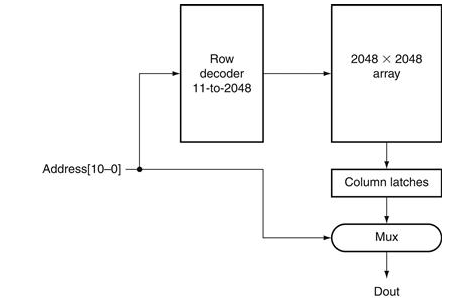
\includegraphics[scale=0.7]{img/dram2.png}
\end{center}
L'entrata sulle righe sceglie un numero di righe e attiva il corrispondente \textit{word line}, il contenuto di tutte le colonne nelle righe attive viene salvato nei Latch. Due segnali, il RAS, \textit{Row Access Strobe}, e il CAS, \textit{Columns Access Strobe}, segnalano quando righe e colonne sono state rifornite con i dati. Questo sistema rende l'accesso alla DRAM più lungo, tra i $50$ e 9 $70$ \textit{ns}. Una DRAM 64M$\times$4 tiene 8K accessi su ogni riga, ma ne salva solo 4 con l'accesso alle colonne
\end{itemize}
\section{ALU}
\textit{arithmetic logic unit} è l'unità che esegue le operazioni aritemica (\textit{add, sub, etc...}) e quelle logiche (\textit{and, or}). La ALU è composta da porte OR, porte NAD, multiplexor e inverter.
\subsection{ALU a 1bit}
ovviamente le operazioni logiche sono più semplici, come si può qui vedere:
\begin{center}
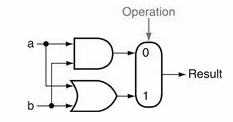
\includegraphics[scale=0.7]{img/alu.png}
\end{center}
si ha un multiplexor a destra che sceglie AND o OR in base al valore di \textit{operation}, 0 per AND e 1 per OR. \\
Vediamo l'addizione. Un sommatore deve avere 2 input e un bit di output per la somma. C'è poi un secondo output, il \textit{CarryOut}, contenente il resto della somma che è collegato come terzo input, \textit{CarryIn}, ad un sommatore vicino (schema in figura). CarryOut e somma possono essere espresse come espressioni logiche, secondo la seguente tabella:
\begin{center}
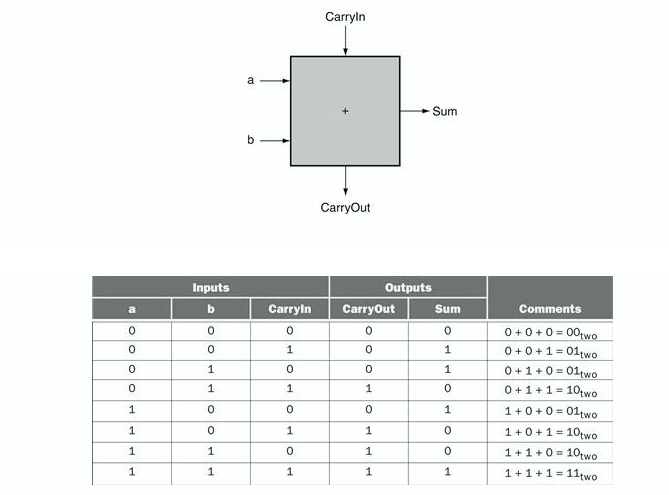
\includegraphics[scale=0.6]{img/alu2.png}
\end{center}
Si ha la seguente espressione dalla tabella per il CarryOut:
$$CarryOut=(b\cdot CarryIn)+(a\cdot CarryIn)+(a\cdot b)+(a\cdot b\cdot CarryIn)$$
Se $a\cdot b\cdot CarryIn$ è true allora anche gli altri tre termini devono esserlo quindi possiamo semplificare:
$$CarryOut=(b\cdot CarryIn)+(a\cdot CarryIn)+(a\cdot b)$$
ottenendo questo circuito per ottenere il CarryOut:
\begin{center}
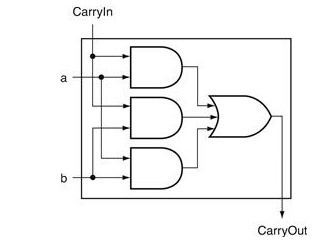
\includegraphics[scale=0.6]{img/alu3.png}
\end{center}
\newpage
La somma normale invece è settata in modo da avere 1 in ouput solo se 1 o 3 ingressi sono 1 con la seguente equazione:
$$sum=(a\cdot \overline{b}\cdot \overline{CarryIn})+(\overline{a}\cdot b\cdot \overline{CarryIn})+(\overline{a}\cdot \overline{b}\cdot CarryIn)+(a\cdot b\cdot CarryIn)$$
Aggiungendo quindi il sommatore del CarryOut allo schema per le equazioni logiche si ottiene:
\begin{center}
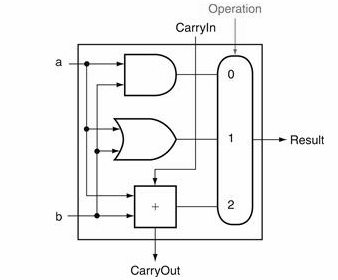
\includegraphics[scale=0.7]{img/alu4.png}
\end{center}
\subsection{ALU a 32bit}
Si ottiene collegando 32 ALU a 1bit ottenendo così 32 risultati possibili. Si può per esempio avere la sottrazione, che consiste nel sommare l'inverso di un operando, aggiungendo 1 per il \textit{complemento a 1}. Per invertire l'operando si aggiunge semplicemente un multiplexor 2:1 che sceglie, per esempio tra $b$ e $\overline{b}$, ottenendo:
\begin{center}
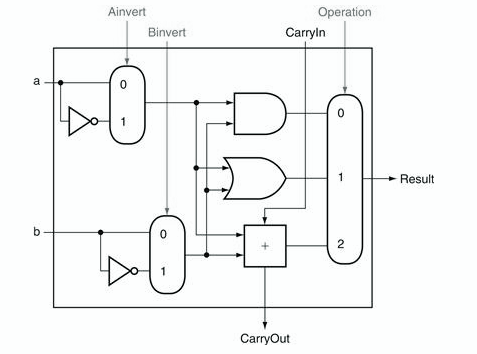
\includegraphics[scale=0.5]{img/alu5.png}
\end{center}
e nel complesso la seguente rappresentazione dell'ALU a 32bit:
\begin{center}
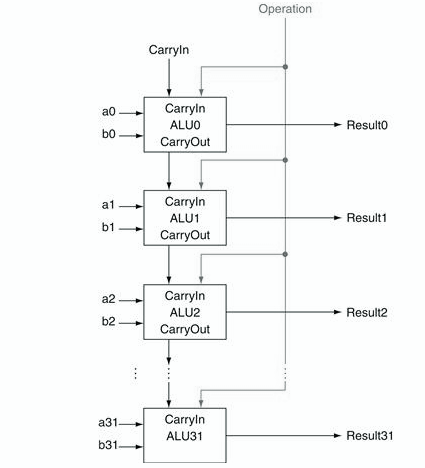
\includegraphics[scale=0.6]{img/alu6.png}
\end{center}
Aggiungiamo ora un'operazione di comparazione, la \textit{slt}, che ha 1 come output se rs<rt o 0 se viceversa. Per farlo si aggiunge l'input \textit{Less} usato solo per questa istruzione, e si connette 0 al bit meno significativo della ALU, si usa così il bit meno significativo unicamente per questa istruzione. Inoltre ora si può calcolare anche un valore negativo, usando il bit più significativo per identificarlo, 1 per un numero negativo e 0 per uno positivo. Dato che il bit più significativo per la slt non è l'output del sommatore si dovrà usare il valore di input Less. Si necessita quindi di un bit aggiuntivo per il bit più significativo che ha un extra output: l'output del sommatore. Si crea quindi un nuovo output del sommatore, detto \textit{set}, usato solo dalla slt. Inoltre si aggiunge l'\textit{overflow detector} apposta per questo bit Più significativo della ALU. Si ha quindi:
\begin{center}
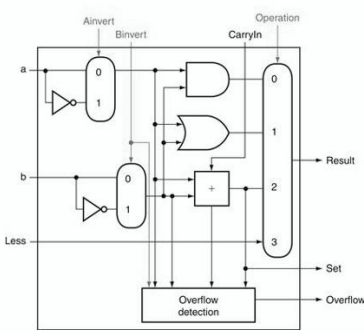
\includegraphics[scale=0.7]{img/alu7.png}
\end{center} 
e nel complesso ecco l'ALU a 32bit, con l'aggiunta del controllo che il risultato sia zero, per testare l'uguaglianza ($zero=\sum_{i=0}^{31} \overline{result-i}$):
\begin{center}
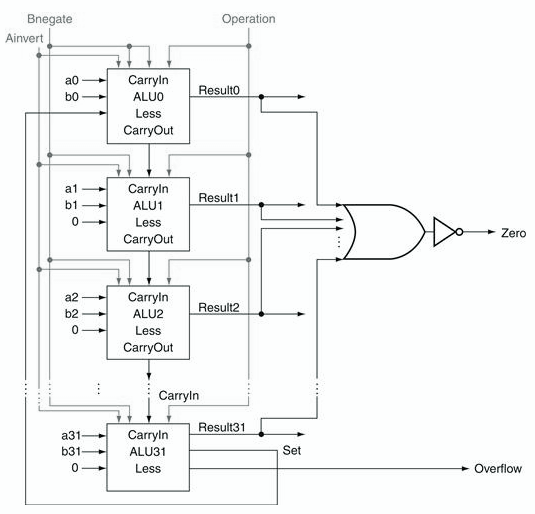
\includegraphics[scale=0.6]{img/alu8.png}
\end{center}
solitamente indicata col seguente simbolo:
\begin{center}
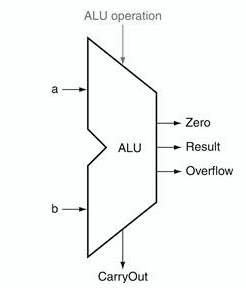
\includegraphics[scale=0.7]{img/alu9.png}
\end{center}
\section{Esercizi}
\begin{esercizio}
Dato il seguente circuito con la seguente tabella di ingressi definire l'output:
\begin{center}
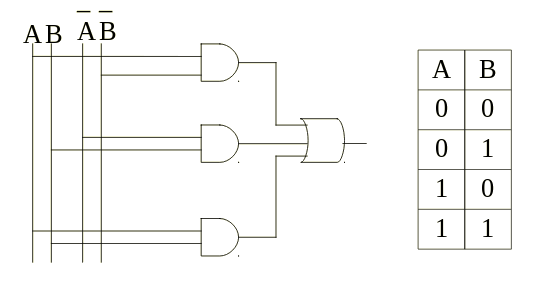
\includegraphics[scale=0.7]{img/es1.png}
\end{center}
Si ha la seguente tabella della verità:
\begin{center}
\begin{tabular}{|c|c|c|c|c|c|c|c|}
\hline 
& & & & & & &\\
$A$ & $B$ & $\overline{A}$ & $\overline{B}$ & $A\wedge\overline{B}$  & $\overline{A}\wedge B$ & $A\wedge B$1 & final $\vee$\\
\hline
0 & 0 & 1 & 1 & 0 & 0 & 0 & 0\\
\hline
0 & 1 & 1 & 0 & 0 & 1 & 0 & 1\\
\hline
1 & 0 & 0 & 1 & 1 & 0 & 0 & 1\\
\hline
1 & 1 & 0 & 0 & 0 & 0 & 1 & 1\\
\hline
\end{tabular}
\end{center}
Quindi come output si avrà in ordine $M=[0,1,1,1]$
\end{esercizio}
\begin{esercizio}
Dato il seguente circuito con la seguente tabella di ingressi definire l'output:
\begin{center}
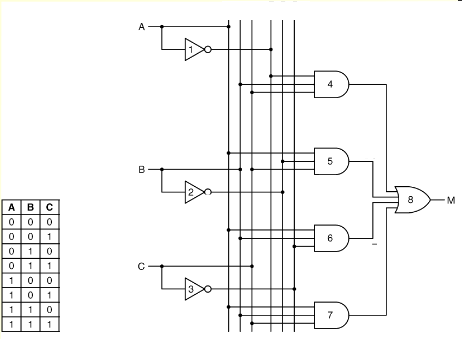
\includegraphics[scale=0.6]{img/es2.png}
\end{center}
Si ha la seguente tabella della verità:
\begin{center}
\begin{tabular}{|c|c|c|c|c|c|c|c|c|c|c|}
\hline 
& & & & & & & & & & \\
$A$ & $B$ & $C$ & $\overline{A}$ & $\overline{B}$ & $\overline{C}$ & $\overline{A}\wedge B\wedge C$  & $A\wedge \overline{B}\wedge C$ & $A\wedge B\wedge\overline{C}$ & $A\wedge B\wedge C$ & final $\vee$\\
\hline
0 & 0 & 0 & 1 & 1 & 1 & 0 & 0 & 0 & 0 & 0\\
\hline
0 & 0 & 1 & 1 & 1 & 0 & 0 & 0 & 0 & 0 & 0\\
\hline
0 & 1 & 0 & 1 & 0 & 1 & 0 & 0 & 0 & 0 & 0\\
\hline
0 & 1 & 1 & 1 & 0 & 0 & 1 & 0 & 0 & 0 & 1\\
\hline
1 & 0 & 0 & 0 & 1 & 1 & 0 & 0 & 0 & 0 & 0\\
\hline
1 & 0 & 1 & 0 & 1 & 0 & 0 & 1 & 0 & 0 & 1\\
\hline
1 & 1 & 0 & 0 & 0 & 1 & 0 & 0 & 1 & 0 & 1\\
\hline
1 & 1 & 1 & 0 & 0 & 0 & 0 & 0 & 0 & 1 & 1\\
\hline
\end{tabular}
\end{center}
Quindi come output si avrà in ordine $M=[0,0,0,1,0,1,1,1]$
\end{esercizio}
\newpage
\begin{esercizio}
Data la seguente tabella con input e output definire la funzione di D (usando gli OR di AND) e disegnare il circuito:
\begin{center}
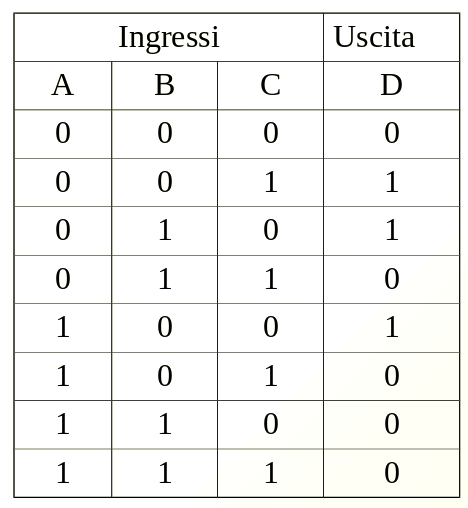
\includegraphics[scale=0.7]{img/es3.png}
\end{center}
Iniziamo scrivendo la tabella di verità con ciò che conosciamo:
\begin{center}
\begin{tabular}{|c|c|c|c|c|c|c|c|c|c|c|}
\hline 
& & & & & & & & & \\
$A$ & $B$ & $C$ & $\overline{A}$ & $\overline{B}$ & $\overline{C}$ & $\wedge \wedge $  & $\wedge \wedge $ & $\wedge \wedge$ & final $\vee$\\
\hline
0 & 0 & 0 & 1 & 1 & 1 &  &  &  &  0\\
\hline
0 & 0 & 1 & 1 & 1 & 0 &  &  &  &  1\\
\hline
0 & 1 & 0 & 1 & 0 & 1 &  &  &  &  1\\
\hline
0 & 1 & 1 & 1 & 0 & 0 &  &  &  &  0\\
\hline
1 & 0 & 0 & 0 & 1 & 1 &  &  &  &  1\\
\hline
1 & 0 & 1 & 0 & 1 & 0 &  &  &  &  0\\
\hline
1 & 1 & 0 & 0 & 0 & 1 &  &  &  &  0\\
\hline
1 & 1 & 1 & 0 & 0 & 0 &  &  &  &  0\\
\hline
\end{tabular}
\end{center}
si avranno 3 doppi AND tra 3 degli elementi delle prime 6 colonne. Dato che l'uscita è formata dall'OR delle prime tre colonne posso intuire che per avere 0 devo avere tutti e tre i campi 0, si ottiene quindi:
 \begin{center}
\begin{tabular}{|c|c|c|c|c|c|c|c|c|c|c|}
\hline 
& & & & & & & & & \\
$A$ & $B$ & $C$ & $\overline{A}$ & $\overline{B}$ & $\overline{C}$ & $\wedge \wedge $  & $\wedge \wedge $ & $\wedge \wedge$ & final $\vee$\\
\hline
0 & 0 & 0 & 1 & 1 & 1 & 0 & 0 & 0 &  0\\
\hline
0 & 0 & 1 & 1 & 1 & 0 &  &  &  &  1\\
\hline
0 & 1 & 0 & 1 & 0 & 1 &  &  &  &  1\\
\hline
0 & 1 & 1 & 1 & 0 & 0 & 0 & 0 & 0 &  0\\
\hline
1 & 0 & 0 & 0 & 1 & 1 &  &  &  &  1\\
\hline
1 & 0 & 1 & 0 & 1 & 0 & 0 & 0 & 0 &  0\\
\hline
1 & 1 & 0 & 0 & 0 & 1 & 0 & 0 & 0 &  0\\
\hline
1 & 1 & 1 & 0 & 0 & 0 & 0 & 0 & 0 &  0\\
\hline
\end{tabular}
\end{center}
quelli con 1 in uscita comportano la presenza di almeno un 1 come risultato di uno dei tre doppi and, per avere 1 in uscita da un doppio end si necessita di avere le 3 entrate uguali a 1. Si nota così che per la seconda riga servono $\overline{A},\overline{B},C$, ottenendo $1,0,0$  per la terza $\overline{A}, B, \overline{C}$, ottenendo $0,1,0$ per la quinta $A, \overline{B}, C$ , ottenendo $0,0,1$ e avendo infine:
\begin{center}
\begin{tabular}{|c|c|c|c|c|c|c|c|c|c|c|}
\hline 
& & & & & & & & & \\
$A$ & $B$ & $C$ & $\overline{A}$ & $\overline{B}$ & $\overline{C}$ & $\overline{A}\wedge \overline{B}\wedge C$  & $\overline{A}\wedge B\wedge\overline{C} $ & $A\wedge \overline{B}\wedge\overline{C}$ & final $\vee$\\
\hline
0 & 0 & 0 & 1 & 1 & 1 & 0 & 0 & 0 &  0\\
\hline
0 & 0 & 1 & 1 & 1 & 0 & 1 & 0 & 0 &  1\\
\hline
0 & 1 & 0 & 1 & 0 & 1 & 0 & 1 & 0 &  1\\
\hline
0 & 1 & 1 & 1 & 0 & 0 & 0 & 0 & 0 &  0\\
\hline
1 & 0 & 0 & 0 & 1 & 1 & 0 & 0 & 1 &  1\\
\hline
1 & 0 & 1 & 0 & 1 & 0 & 0 & 0 & 0 &  0\\
\hline
1 & 1 & 0 & 0 & 0 & 1 & 0 & 0 & 0 &  0\\
\hline
1 & 1 & 1 & 0 & 0 & 0 & 0 & 0 & 0 &  0\\
\hline
\end{tabular}
\end{center}
\newpage
Ed ecco il circuito:
\begin{center}
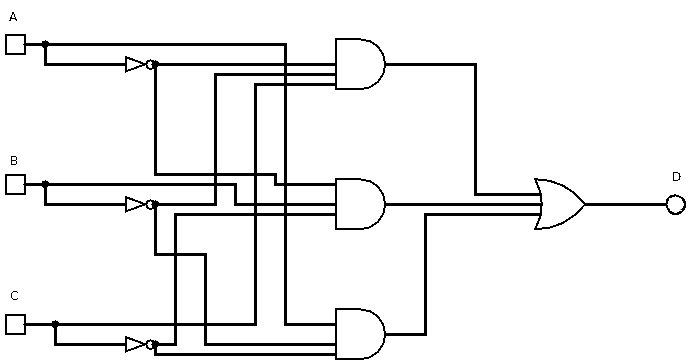
\includegraphics[scale=0.65]{img/es4.png}
\end{center}
\end{esercizio}
\begin{esercizio}
\begin{itemize}
\item un multiplexor a 32 ingressi quanti ingressi di selezione deve avere?\\
Si devono avere $log_2(32)=5$ ingressi di selezione
\item un decoder con 1024 possibili uscite ha un ingresso di quanti bit?\\
Si ha $2^x=1024$ quindi $x=10$ bit in ingresso
\item Considerando una RAM contenente 4096 Kbit la cui 
parola di memoria è di 32 bit, un indirizzo per tale 
memoria da quanti bit è composto?\\
$$4096\,\,Kbit=2^{12}\,\,Kbit = 2^{22} \,\,bit$$
L'altezza della memoria: 
$$\frac{2^{22}}{32}=2^17$$
Ogni indirizzo di questa memoria è rappresentato su 17 bit
\item Considerando una RAM contenente 10 bit e un indirizzo di memoria di 3 bit, da quanti bit è composta una parola di memoria?\\
Larghezza ram = dimensione / numero di parole indirizzabili:
$$\frac{10}{2^3}=1,2$$
quindi una word ha 2 bit (la memoria è composta da 5 parole di memoria e 3 indirizzi non vengono usati)
\item Con 30 bit per un indirizzo di memoria e una parola di 
memoria di 64 bit, qual è la dimensione massima di 
memoria indirizzabile in MB?\\
$$\frac{x}{2^{30}}=64\longrightarrow x= 64\cdot 2^30=6,87\times 10^{10}\,bit $$
divido per 8 e ottengo i byte, per 1024 e ottengo i Kilobyte e per 1024 ancora e ottengo 8192 Megabyte
\end{itemize}
\end{esercizio}
\chapter{Assembly}
Prima di tutto analizziamo cosa accadde quando si compila un programma di alto livello:
\begin{itemize} 
\item il compilatore trasforma il programma in linguaggio assembler, una forma simbolica di ciò che il calcolatore è in grado di interpretare 
\item l'assemblatore traduce il linguaggio assembler in linguaggio macchina. L'hardware MIPS si assicura che \$zero contenga sempre il valore 0 e permette il caricamento di un registro di costanti a 32bit, nonostante il limite a 16bit per le I-Type. L'assemblatore accetta numeri in diverse basi. SI converte quindi il programma assembler in un \textit{file oggetto}, ovvero una sequenza di istruzioni in linguaggio macchina, dati e informazioni necessarie a collocare le istruzioni in memoria nella posizione corretta. L'assemblatore deve determinare gli indirizzi corrispondenti a tutte le etichette, e ne tiene traccia nei salti e nei trasferimenti dati scrivendole in una \textit{tabella dei simboli} che conterrà coppie di tipo \textit{simbolo-indirizzo}
\item per evitare di dover ripetere da 0 tutte le operazioni indicate ogni volta che si cambia qualcosa nel sorgente. Per ovviare a questo problema si è deciso di compilare separatamente ogni procedura e si è creato un programma di sistema chiamato \textit{Linker (Link Editor)} che prende tutte le procedure e le unisce. Avvengono 3 passaggi:
\begin{enumerate}
\item il Linker inserisce in memoria in modo simbolico il codice e i moduli dati
\item determina gli indirizzi dei dati e delle etichette che compaiono nelle istruzioni 
\item corregge i riferimenti interni ed esterni
\end{enumerate}
il Linker utilizza le informazioni di rilocazione e la tabella dei simboli di ciascun modulo oggetto per risolvere le etichette non definite, che si trovano nei salti e nei salti incondizionati. Nel complesso si può dire che trova gli indirizzi vecchi e li sostituisce con quelli nuovi. Si ha che è più veloce correggere in questa maniera il codice piuttosto che ricompilarlo e riassemblarlo. Dopo che tutti i riferimenti esterni sono stati risolti il Linker determina le locazioni di memoria che ciascun modulo dovrà occupare. Quando un Linker inserisce un modulo in memoria tutti i riferimenti \textit{assoluti} (ovvero quelli non definiti in relazione ad un registro) devono essere rilocati in modo da poter riflettere la loro posizione reale. Il Linker procuce un \textit{file eseguibile} eseguibile su un calcolatore, che ha le stesso formato di un \textit{file oggetto} ma non contiene più riferimenti irrisolti (questo passaggio può essere eseguito in maniera parziale con indirizzi non risolti, come nel caso delle librerie).

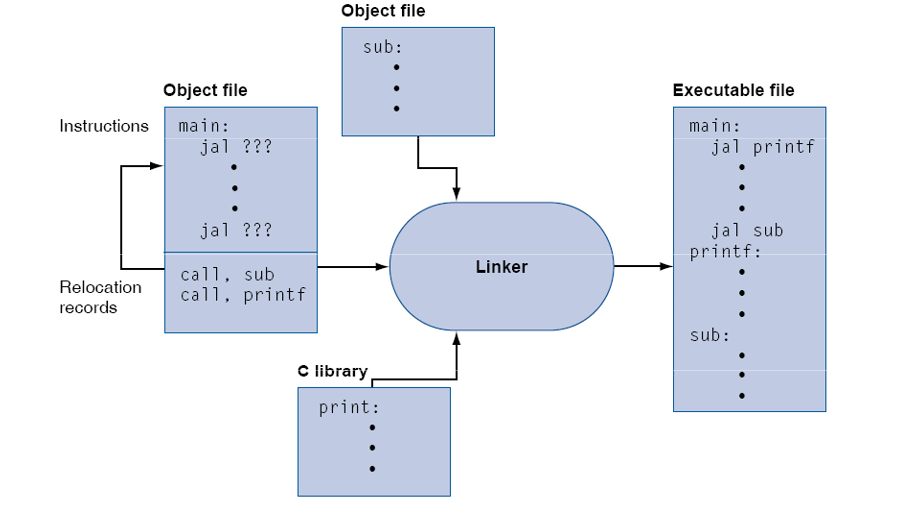
\includegraphics[scale=0.5]{img/linker.png}

\item una volta che l'eseguibile è salvato su disco il sistema operativo può leggero, trasferirlo in memoria ed eseguirlo. Si ha il programma di caricamento, il Loader, che effettua i seguenti passaggi:
\begin{enumerate}
\item lettura dell'intestazione dell'eseguibile per determinare la lunghezza del segmento testo e del segmento dati
\item creazione di uno spazio di indirizzamento sufficiente per testo e dati
\item copia di istruzioni e dati dal file alla memoria
\item copia nello stack degli eventuali parametri passati al programma principale
\item inizializzazione dei registri del calcolatore e impostazione dello stack pointer affinché punti alla prima locazione libera
\item  salto ad una procedura di avvio, \textit{startup}, che copia i parametri nei registri argomento e chiama la procedura principale del programma (\textit{main}), quando quest'ultima restituisce il controllo la procedura di \textit{startup} termina il programma con una chiamata alla funzione di sistema \textit{exit} 
\end{enumerate}
\end{itemize}
Tornando a parlare di CPU si hanno 2 filosofie di progetto:
\begin{itemize}
\item \textbf{RISC (Reduced Instruction Set Computing):} qui si hanno poche istruzioni semplici, una struttura circuitalmente semplice, l'esecuzione veloce di ogni singola istruzione ma occorrono più istruzioni per fare cose anche semplici. Come esempi abbiamo MIPS, ARM o PowerPc.
\item \textbf{CISC (Complex Instruction Set Computing):} qui si hanno istruzioni complesse, struttura circuitale complicata, esecuzione più lenta di ogni singola istruzione ma occorrono meno istruzioni. Come esempi abbiamo Intel x86 (Pentium etc..)
\end{itemize}
Iniziamo a vedere MIPS. Si hanno 32 registri di 32bit e istruzioni di 32bit. Si hanno manipolazioni di dati solo sui registri, si può avere il trasferimento dei dati dalla memoria hai registri e si possono avere alterazioni del flusso di controllo con i \textit{salti}.\\
Iniziamo con qualcosa di semplice:
\textit{somma=a+a+a+a} e \textit{a} si trova nel registri \$8:
\begin{verbatim}
add $9, $8, $8 # metto nel registro $9 la somma a+a
add $9, $9, $9 # metto nel registro $9 la somma (a+a)+(a+a),
                 in quanto (a+a) e nel registro $9
\end{verbatim}
\newpage
vediamo anche le operazioni semplici di \textit{load word}:
\begin{verbatim}
lw $10, 4($8) # carica nel registro $10 il contenuto della
                parola (a 32bit) contenuta all'indirizzo di 
                memoria ottenuto come somma del registro $8
                e dell'offset immediato 4
\end{verbatim}
e \textit{store word}:
\begin{verbatim}
sw $10, 4($8) # memorizza il contenuto del registro $10 
                parola (a 32bit) all'indirizzo di 
                memoria ottenuto come somma del registro $8
                e dell'offset immediato 4
\end{verbatim}
vediamo un esempio più complesso:\\
\textit{i valori delle variabili a,b,c e d sono memorizzati nella memoria partendo dall'indirizzo specificato dal registro \$s0. Aggiungo il valore immediato 10 a tutte le variabili e le salvo in memoria: }
\begin{verbatim}
lw $t0, 0($s0)    # carico in $t0 il contenuto di $s0, senza 
                    nessun offset, ora $t0 è a
addi $t0, $t0, 10 # aggiungo 10 ad a
sw $t0, 0($s0)    # salvo il valore in memoria nel registro
                    $s0
lw $t0, 4($s0)    # carico in $t0 il contenuto del registro 
                    ottenuto con un offset di 4 da $s0, 
                    ora $t0 è b
addi $t0, $t0, 10 # aggiungo 10 a b
sw $t0, 4($s0)    # salvo il valore in memoria nel registro
                    $s0 con un offset di 4
lw $t0, 8($s0)    # carico in $t0 il contenuto del registro 
                    ottenuto con un offset di 8 da $s0, 
                    ora $t0 è c
addi $t0, $t0, 10 # aggiungo 10 a c
sw $t0, 8($s0)    # salvo il valore in memoria nel registro
                    $s0 con un offset di 8
lw $t0, 12($s0)    # carico in $t0 il contenuto del registro 
                    ottenuto con un offset di 12 da $s0, 
                    ora $t0 è d
addi $t0, $t0, 10 # aggiungo 10 a d
sw $t0, 8($s0)    # salvo il valore in memoria nel registro
                    $s0 con un offset di 12
 
\end{verbatim}
\newpage
ecco un altro breve codice:
\textit{calcolo la somma del valore 10, memorizzato in \$s1 e del valore 20 memorizzato nella allocazione di memoria specificata da \$s0 con un offset di 56 byte. Il risultato va memorizzato nella memoria che si trova 3 word più avanti rispetto alla locazione attuale del secondo operando}:
\begin{verbatim}
lw $t0, 56($s0)   # carico in $t0 il contenuto del registro 
                  ottenuto con un offset di 56 byte da $s0
add $t1, $s1, $t0 # faccio la somma tra 10, contenuto in $s1
                    e 20, caricato nella riga precedente in $t0
                    e metto il risultato in $t1
sw $t1, 68($s0)   # salvo la somma nell'indirizzo di memoria
                    ottenuto con un offset di 56 byte, quello
                    del secondo operando, sommato di 3 word
                    ovvero sommato di 12 byte, quindi avrò
                    un offset di 56+12=68
\end{verbatim}
\newpage
introduciamo i flussi di controllo \textit{if-else}:\\
\textit{scrivo in MIPS il seguente codice java:}
\begin{verbatim}
if(i==j)
  f=g+h
else
  f=g-h
\end{verbatim}
considerando che le 5 variabili sono agli indirizzi compresi tra \$s0 e \$s4. L'indirizzo della prima istruzione è 80000:
\begin{verbatim}
80000 bne $s3, $s4, ELSE      # branch if not equal, se $s3 (i) 
                                e $s4 (j) non sono uguali salta
                                all'etichetta ElSE
80004 add $s0, $S1, $s2       # se non si è saltato a ELSE, 
                                ovvero i valori in $s3 e $s4 sono
                                uguali, esegui la somma tra $s1 (g)
                                e $s2 (h) e salvala in $s0 (f)
80008 j EXIT                  # se è stata effettuata la somma salta 
                                all'istruzione exit
80012 ELSE: sub $s0, $S1, $s2 # l'etichetta ELSE riporta la sua
                                istruzione, ovvero la sottrazione
                                tra gli stessi indirizzi della 
                                somma che si avrebbe avuto
                                se fossero stati uguali i e j.
                                Si arriva a questa istruzione 
                                grazie al primo bne, se i e j sono diversi
80016 EXIT: ...               # si esce dal programma, si arriva 
                                qui col jump alla terza riga
                                se si è effettuata la somma o
                                dopo la sottrazione
\end{verbatim}
elenchiamo le istruzioni I-Type di tipo \textit{branch}:
\begin{itemize}
\item \textbf{beq}: \textit{branch on equal}, va al target definito dall'etichetta se i due registri contengono lo stesso valore
\item \textbf{bne}: \textit{branch if not equal}, va al target definito dall'etichetta se i due registri contengono valori diversi
\item \textbf{bgez} \textit{Branch on greater than or equal to zero} va al target definito dall'etichetta se il valore è maggiore uguale di zero
\item \textbf{bgtz} \textit{Branch on greater than zero} va al target definito dall'etichetta se il valore è maggiore di zero
\item \textbf{blez} \textit{Branch on less than or equal to zero} va al target definito dall'etichetta se il valore è minore uguale di zero
\item \textbf{bltz} \textit{Branch on less than zero} va al target definito dall'etichetta se il valore è minore di zero
\item \textbf{bgezal} \textit{Branch on greater than or equal to zero and link} va al target definito dall'etichetta se il valore è maggiore uguale di zero e salva l'indirizzo del return in \$31
\item \textbf{bltzal} \textit{Branch on less than or equal to zero and link} va al target definito dall'etichetta se il valore è minore uguale di zero e salva l'indirizzo del return in \$31
\end{itemize}
Prima di continuare è necessario analizzare gli scopi dei vari registri. Ecco una comoda tabella:\\
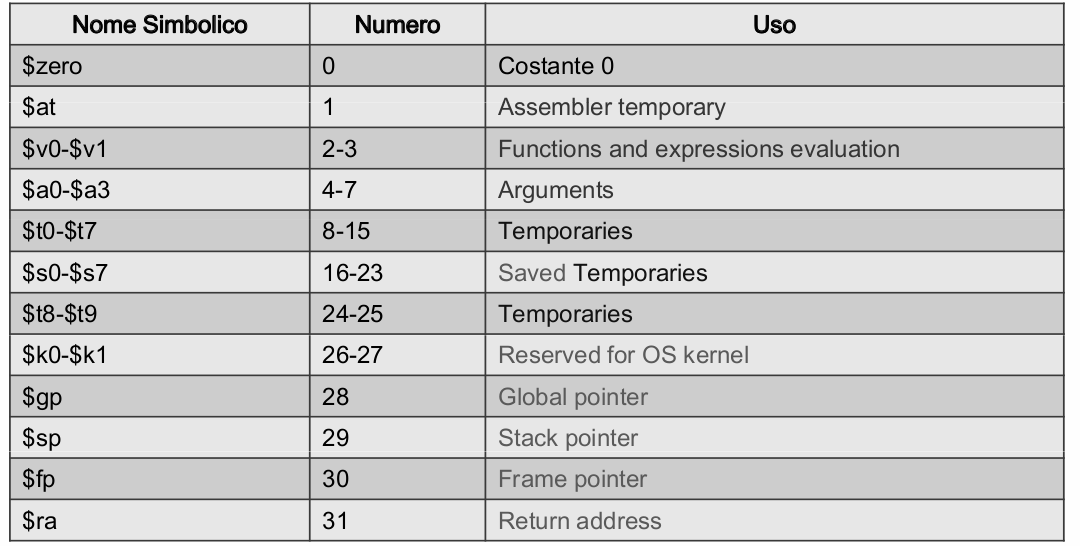
\includegraphics[scale=0.4]{img/regmips.png}\\
Tutti i registri il cui uso è scritto in grigio chiaro sono usati da assembler, compilatore e sistema operativo (ovvero tutti tranne i \$tn, parte dei \$sn e \$zero) e sono da trattare con cautela.\\
\newpage
Programmando in assembly si possono avere le direttive date all'assembler per consentirgli di, per esempio:
\begin{itemize}
\item associare etichette simboliche ad indirizzi
\item allocare spazi di memoria per le variabili
\item decidere in quali zone di memoria allocare istruzioni e dati
\end{itemize}
vediamo quale esempio di direttive:
\begin{itemize}
\item \textit{.data} $<$\textit{addr}$>$, quel che segue va nel segmento dati, eventualmente all'indirizzo addr
\item \textit{.byte b1,...,bn} inizializza i valori in byte successivi
\item \textit{.word w1,...,wn} inizializza i valori in word successive
\item \textit{.text} $<$\textit{addr}$>$, quel che segue va nel segmento text (programma), eventualmente all'indirizzo addr
\end{itemize}
vediamo un esempio "completo":
\begin{verbatim}
      .data
item: .word 1
      .text
      .globl main
main: lw $t0,item
\end{verbatim}
analizziamo ora qualche istruzione aritmetica e logica:
\begin{itemize}
\item \textit{add rd, rs, rt:} è l'addizzione, \textit{rd=rs+rt}, può andare in overflow
\item \textit{addi rd, rs, imm:} è l'addizione immediata, \textit{rd=rs+imm} (con imm che può essere negativo), può andare in overflow
\item \textit{and rd, rs, rt:} è l'\textit{and bit a bit} di \textit{rs} e \textit{rt}, col risultato salvato in \textit{rd}
\item \textit{andi rd, rs, imm:} è l'\textit{and bit a bit} di \textit{rs} e imm (esteso anche a 0), col risultato salvato in \textit{rd}
\item \textit{or rd, rs, rt:} è l'\textit{or bit a bit} (logical \textit{or}) di \textit{rs} e \textit{rt}, col risultato salvato in \textit{rd}
\item \textit{ori rd, rs, imm:} è l'\textit{or bit a bit}(logical \textit{or}) di \textit{rs} e imm (esteso anche a 0), col risultato salvato in \textit{rd}
\item \textit{sll rd, rt, shamt:} è lo \textit{shift left} di \textit{rd} della distanza \textit{shamt}, col risultato in \textit{rd}
\item \textit{lui rt, imm:} è \textit{load upper immediate}, carica i 16bit del valore immediato nei 16bit più significativi di \textit{rt} e i rimanenti 16bit meno significativi vengono messi a 0. Se si vuole salvare un valore a 32bit prima si fa \textit{lui \$s0, imm1}, con \textit{imm1} decimale che rappresenta i primi 16bit del valore, caricando quindi i 16bit più significativi (quelli a sinistra), e poi si fa \textit{ori \$s0, \$s0, imm2}, con \textit{imm2} che rappresenta il decimale dei secondi 16bit, caricando i 16bit meno significativi (quelli a destra)
\end{itemize}
Si hanno poi le \textit{pseudo istruzioni}, istruzioni assembly che non hanno una corrispondente istruzione macchina che vengono tradotte dall'assembler in una sequenza di istruzioni. Per esempio di può avere \textit{li rd, imm}, ovvero \textit{load immediate} che carica una costante di 32bit in \textit{rd} (esempio \textit{li \$s0, 4000000} che l'assemblatore traduce in \textit{lui \$s0, 61; ori \$s0, \$s0, 2304}). Un altro esempio può essere \textit{move \$t0, \$t1}, che sposta il contenuto di \$t1 in \$t0, che l'assemblatore traduce con \textit{add \$t0, \$zero, \$t1}, somma a \$t1 zero e lo salva in \$t0.
Vediamo un esercizio:\\
\textit{si leggano 3 valori a,b e c memorizzati all'etichetta valori nei registri \$t0, \$t1 e \$t2. Calcolo la somma dei 3 in \$s0 se il primo è positivo, il prodotto se il primo è negativo e l'AND se è uguale a 0. memorizzo il risultato nella locazione subito dopo il terzo valore}
\begin{verbatim}
        .data
valori: .word 0, 5, 2
        .word 0
        .text
        .globl main
        
main:   la $t7, valori       # i valori si troveranno a partire dal registro $t7

        lw $t0, 0($t7)       # carico i valori in $t0, $t1 e $t2
                               usando i vari offstet a step di 4
        lw $t1, 4($t7) 
        lw $t2, 8($t7)  
        
        bgt $t0, $zero, than # se il valore di $t0 è positivo
                               vado all'etichetta than
        blt $t0, $zero, else # se il valore di $t0 è negativo
                               vado all'etichetta else
        
        and $s0, $t1, $t2    # se arrivo qui significa che $t0 è 0
                               quindi calcolo l'AND tra $t1 e $t2
                               e salvo in $s0
        j fine               # dopo il calcolo dell'and salto all'etichetta fine
else:   mul $s0, $t0, $t1    # calcolo il prodotto dei contenuti dei
                               tre registri se $t0<0
        mul $s0, $s0, $t2
        j fine               # salto all'etichetta fine 
than:   add $s0, $t0, $t1    # calcolo la somma dei contenuti dei
                               tre registri se $t0>0
        add $s0, $s0, $t2
        j fine               # salto all'etichetta fine
fine:   sw $s0, 12($t7)      # alla fine salvo nella locazione dopo
                               il terzo valore, quindi con un offset di 12
                               da $t7 
\end{verbatim}
Ecco un altro esercizio:
\textit{calcolo la lunghezza di una stringa memorizzata dall'indirizzo \textbf{stringa}. La stringa finisce col carattere $\backslash 0$. Salvo la dimensione della stringa in memoria dopo la stringa in un word:}
\begin{verbatim}
          .data
stringa:  .asciiz "Hello World!" # definisco la stringa
                                   13 byte per la stringa
                                   12 byte per la lunghezza
dim:      .word 0
charfine: .asciiz ""             # char finale
          .text
          .globl main
        
main:     la $t0, stringa        # carico in $t0 l'indirizzo della stringa
          add $t2, $zero, $zero  # definisco un contatore
          la $s5, charfine       # carico in $t0 l'indirizzo di charfine
          lb $s1, 0$($s5)        # load byte, metto in $s1 il contenuto
                                   di $s5: ""
ciclo:
          lb $s7, 0($t0)         # carico il $s7 il char 0 della stringa
          beq $s7, $s1, fine     # se $s7 è uguale a $s1, ovvero a ""
                                   salta a fine
          addi $t2, $t2, 1       # incrementa il contatore
          addi $t0, $t0, 1       # incremento di un char
          j ciclo                # torno ad inizio ciclo
                                   dove in $s7 ci sarà il char successivo
fine:     la $t3, dim            # carico in $t3 l'indirizzo di dim
          sw $t2, 0($t3)         # carico il risultato in $t3
\end{verbatim}
Un altro esercizio:
\textit{Calcolo il minimo tra a,b e c memorizzati nella memoria all'etichetta "numeri". Salvo all'etichetta "minimo:}
\begin{verbatim}
          .data
numeri:   .word 9, 7, 8
minimo:   .word 0
          .text
          .globl main
          
main:     .la $s0, numeri
          .la $s1, minimo
          .lw $t0, 0($s0)
          .lw $t1, 4($s0)
          .lw $t2, 8($s0)
          
          blt $t0, $t1, AminB # verifico se a<b, se vero vado a AminB
          blt $t1, $t2, BminC # verifico se b<c, se vero vado a BminC
          move $t3, $t2       # se arrivo qui ho b<a e c<b, quindi c 
                                è il minimo, e lo salvo in $t3
          j salvamin
BminC:    move $t3, $t1       # se in main arrivo a BminC
                                significa che b<a e b<c
                                quindi b è il minimo e lo salvo
          j salvamin
AminB:    blt $t0, $t2, AminC # verifico se a<c, se vero vado a AminC
          move $t3, $t2       # se arrivo qui ho a<b e c<a,
                                c è il minimo e lo salvo
          j salvamin
AminC:    move $t3, $t0       # se arrivo qui ho a<b e a<c,
                                a è il minimo e lo salvo       
salvamin: sw $t3, 0($s1)      # salvo $t3 in minimo
\end{verbatim}
Iniziamo a vedere come funzionano le procedure. Introduciamo delle istruzioni utili:
\begin{itemize}
\item \textit{jal <IndirizzoProcedura>:} \textit{jump and link}, salva nel registro 31 \$ra, detto \textit{return address} l'indirizzo a cui tornare dopo la procedura, ovverlo l'indirizzo successivo (+4) a quello della \textit{jal}
\item \textit{jr <registro>:} \textit{jump register}, salta all'indirizzo contenuto in un registro, constente di saltare a qualsiasi locazione di memoria. \textit{jr \$ra} è uno degli utilizzi tipici, esegue il ritorno da una procedura saltando all'indirizzo precedentemente salvato da \textit{jal}
\end{itemize}
Si hanno delle convenzioni base, si hanno infatti dei registri usati apposta dalle procedure:
\begin{itemize}
\item \textit{\$a0-\$a3} sono i registri argomento per il passaggio di parametri
\item \textit{\$v0-\$v1} sono i registri valore per la restituzione dei risultati
\end{itemize}
Un parametro può essere sia un dato che un indirizzo. Vediamo qualche esempio elementare:
\\
\textit{programma che definisce 4 numeri, definisce una procedura somma1 che riceve due numeri e fa la somma, viene chiamata prima tra num1 e num2 salvando in result1 e poi tra num3 e num4 salvando in result2}
\begin{verbatim}
         .data
num1:    .word 50
num2:    .word 14
result1: .word 0
num3:    .word 50
num4:    .word -66
result2: .word 0
         .text
         .globl main

main:    lw $a0, num1      # carico in $a0 num1
         lw $a1, num2      # carico in $a1 num2
         jal somma1        # l'indirizzo della prossima istruzione viene
                             salvato in $ra e si salta alla procedura
         sw $v0, result1   # salvo result1
         
         lw $a0, num3      # carico in $a0 num3
         lw $a1, num4      # carico in $a1 num4
         jal somma1        # l'indirizzo della prossima istruzione viene
                             salvato in $ra e si salta alla procedura
         sw $v0, result2   # salvo result2
somma1:  add $v0, $a0, $a1 # secondo le convenzioni viste sopra
         j $ra             # $ra contiene l'indirizzo di ritorno
\end{verbatim}
\newpage
In una situazione reale si deve tenere conto anche del sistema operativo, che è un insieme di programmi che stanno in un'area protetta della memoria e svolgono funzioni di utilità generale (esempio I/O), richiamabili dai programmi utente. Alcune funzioni base possono essere richiamate col meccanismo di \textit{syscall}, concettualmente analogo alle procedure.Si ha la seguente tabella con le convenzioni per le syscall:
\begin{center}
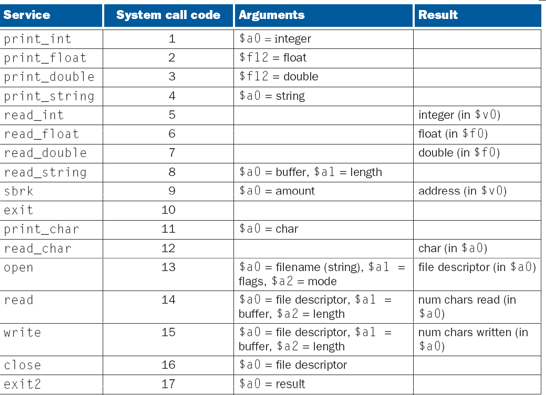
\includegraphics[scale=0.6]{img/syscall.png}
\end{center}
si imposta i \$v0 il codice della chiamata e i parametri nei registri \$a0-\$a3. Facciamo qualche esempio:\\
\textit{codice che stampa "la risposta è 5":}
\begin{verbatim}
        .data
str:    .asciiz "la risposta è"  
numero: .word 5

        .text
        li $v0, 4      # codice per la syscall print_str
        la $a0, str    # indirizzo della stringa da stampare
                         passato per indirizzo
        syscall        # stampa la stringa
        
        li $v0, 1      # codice per la syscall print_int
        lw $a0, numero # numero da stampare passato per valore
        syscall        # stampa il numero
       
\end{verbatim}
\newpage
Torniamo a parlare dei registri, soprattutto dell'uso dei registri all'interno di procedure. Si hanno convenzioni per i \$t e i \$s:
\begin{itemize}
\item \textit{\$t:} sono i registri \textit{temporary} e non sono salvati dalla procedura. Il chiamante non si può aspettare di trovarli immutati dopo una procedura e devono essere salvati prima della chiamata a procedura
\item \textit{\$s:} sono i registri \textit{saved} e sono salvati dalla procedura. Il chiamante ha diritto di aspettarsi che siano immutati dopo una chiamata a procedura. Se la procedura usa questi registri si deve salvarne il contenuto all'inizio e ripristinarlo dopo, grazie all'uso dello stack
\end{itemize}
Si distinguono due tipi di procedure:
\begin{enumerate}
\item \textit{procedure foglia:} procedure che non chiamano altre procedure
\item \textit{procedure non foglia:} procedure che chiamano altre procedure, in questo caso bisogna far si che una procedura \textit{non foglia} salvi il contenuto in \$ra e lo ripristini prima del ritorno
\end{enumerate}
Vediamo il comportamento di una procedura dal punto di vista dello \textit{stack}, infatti alloca spazio nello \textit{stack}: 
\begin{itemize}
\item  decrementa \$sp per lasciare nello \textit{stack} lo spazio necessario al salvataggio, 1 word per ogni registro da salvare
\item salva \$ra
\item salva eventuali altri registri usando \$sp come registro base
\item ripristina i registri
\item incrementa \$sp per riportarlo alla situazione iniziale
\item si torna alla procedura \textit{jr \$ra}
\end{itemize}
\begin{center}
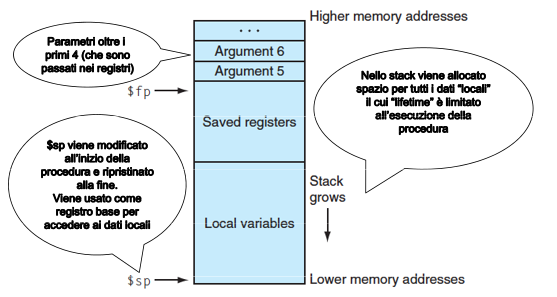
\includegraphics[scale=0.55]{img/stack.png}
\end{center}
\begin{center}
\includegraphics[scale=0.65]{img/stack2.png}
\end{center}
Un frame di stack (\textit{chiamata di procedura}) è un blocco di memoria associata alla procedura. \$sp punta alla prima parola del frame, \$fp all'ultima e un frame di solito è un multiplo della parola doppia (8 byte). Per esempio un frame di 32 byte:
\begin{verbatim}
addi $sp, $sp. -32 # frame di stack di 32 byte, pop dello stack
addi $fp, $sp, 28  # imposta il frame pointer
sw $ra, 0($fp)     # salva l’indirizzo di ritorno come primo
                     word nel frame sullo stack, push nello stack
\end{verbatim}
Vediamo qualche esempio pratico:\\
\textit{vediamo un main che chiama proc1 che a sua volta chiama proc2, stampando i vari punti}
\begin{verbatim}
      .data
msg1: .asciiz "esecuzione del Main...\n"
msg2: .asciiz "esecuzione Proc1...\n"
msg3: .asciiz "esecuzione Proc2...\n"
msg4: .asciiz "fine Proc2.\n"
msg5: .asciiz "fine Proc1.\n"
msg6: .asciiz "fine Main.\n"
      .globl main
      
      .text
main:  
      li $v0, 4         # stampa msg1
      la $a0, msg1
      syscall
      
      jal proc1         # $ra contiene l'indirizzo dell'etichetta
      
      
rientromain:
      li $v0, 4         # stampa msg6
      la $a0, msg6
      syscall
      li $v0, 10        # syscall exit
      syscall
      
proc1:
      li $v0, 4         # stampa msg2
      la $a0, msg2
      syscall
      addi $sp, $sp, -4 # faccio spazio sullo stack
      sw $ra, 0($sp)    # pusho $ra e salvo il punto di rientro
                          del chiamante
      jal proc2

rientro1:
      lw $ra, 0($sp)    # recupero il valore corretto di $ra
      addi $sp, $sp, 4  # eseguo il pop dello stack
      li $v0, 4         # stampa msg5
      la $a0, msg5
      syscall
      jr $ra            # restituisco il controllo al chiamante
     
proc2:
      li $v0, 4         # stampa msg3
      la $a0, msg3
      syscall
      
      li $v0, 4         # stampa msg4
      la $a0, msg4
      syscall
      jr $ra            # restituisco il controllo al chiamante
\end{verbatim}
\textit{Considero un array di 8 word, ogni elemento dell'array rappresenta una cifra binaria (0 o 1) di un numero binario. Implemento una procedura  CA2 che lascia invariati tutti gli zeri e il primo 1 partendo dall'ultimo elemento dell'array e inverte tutti gli altri. Implemento una procedura INVERTI che inverte 0 in 1 e viceversa. CA2 chiama INVERTI:}
\begin{verbatim}
        .data
numero: .word 0, 1, 0, 1, 1, 0, 0, 0
        .text
        .globl main
        
main:   la $a0, numero
        jal CA2                # vado a CA2
        li $v0, 17             # syscall per exit2
        syscall
        
CA2:    li $t5, 8              # carica la dimensione dell'array
        addi $t0, $a0, 28      # carico in $t0 l'ultimo elemento dell'array
        
ciclo1: bltz $t5, fine1        # va a fine 1 se $t5 è minore di 0
        lw $t7, 0($t0)         # carico in $t7 l'ultimo elemento
        addi $t5, $t5, -1      # decresco $t5 di 1 ad ogni ciclo, 
                                 parte da 8
        addi $t0, $t0, -4      # decresco l'indirizzo che mi indica il binario
        beq $t7, $zero, ciclo1 # se $t7 è 0 si riprende il ciclo1
                                 se no si va al ciclo2
ciclo2  beqz $t5, fine1        # se non ci sono più elementi si va 
                                  alla fine
        la $a0, 0($t0)
        addi $sp, $sp, -4      # faccio spazio nello stack
        sw $ra, 0($sp)         # pusho $ra
        
        jal INVERTI
        
        lw $ra, 0($sp)         # recupero il valore corretto di $ra
        addi $sp, $sp, 4       # eseguo il pop dello stack
        
        addi $t5, $t5, -1      # decremento la posizione degli elementi
        addi $t0, $t0, -4      # decremento l'indirizzo che mi indica il binario
        j ciclo2

fine1:  jr $ra                 # restituisco il controllo al chiamante


INVERTI:
         lw $t3, 0($a0)        # carico il parametro passato
         bgtz $t3, uno         # se il parametro è maggiore uguale
                                 di zero vado alla procedura uno
         addi $t3, $t3, 1      # se arrivo qua significa che il
                                 valore è 0, aggiungo 1 per invertire
         j fine2
uno:     addi $t3, $t3, -1     # se arrivo qua significa che il
                                 valore è 1, tolgo 1 per invertire
  
fine2:   sw $t3, 0($a0)        # ripristino $t3
         jr $ra                # restituisco il controllo al chiamante

\end{verbatim}
\chapter{Datapath} 
Si vedrà come costruire un'unità di elaborazione dati (\textit{datapath}) e l'unità di controllo associata a 2 diverse implementazioni hardware dell'insieme di istruzioni MIPS. Si vedrà innanzitutto un'interpretazione che comprende le istruzioni base del MIPS (\textit{lw, sw, add, sub, and, or, slt, beq, j}. Si escludono molte istruzioni e si esclude l'uso di numeri in virgola mobile. Molti componenti necessari per realizzare queste istruzioni sono i medesimi, per esempio i primi due passi sono sempre identici:
\begin{enumerate}
\item inviare il contenuto del program counter (\textit{PC}) alla memoria che contiene il programma e prelevare l'istruzione dalla memoria. Questa operazione è chiamata \textit{fetch} ("raggiungere")
\item leggere il contenuto di uno o due registri utilizzando i campi dell'istruzione per selezionare in registri. Per \textit{lw}, per esempio, serve un solo registro ma la maggior parte delle istruzioni ne richiede 2
\end{enumerate}
dopo questi due passi le azioni richieste variano da istruzione a istruzione, dividendosi però in macrogruppi, dove le azioni sono simili:
\begin{itemize}
\item istruzioni di accesso alla memoria (\textit{lw, sw, etc...})
\item istruzioni aritmetico logiche (\textit{add, sub, and, or, slt, etc...})
\item istruzioni di salto (\textit{beq, j, etc...})
\end{itemize} 
Tranne i salti incondizionati tutte le istruzioni usano l'unità aritmetico.logica (\textit{ALU}) dopo aver letto i registri: 
\begin{itemize}
\item le istruzioni di accesso alla memoria usano l'ALU per il calcolo dell'indirizzo
\item le istruzioni aritmetico-logiche usano l'ALU per l'esecuzione dell'operazione 
\item le istruzioni di salto usano l'ALU per i confronti
\end{itemize}
Dopo l'uso dell'ALU le azioni variano a seconda delle istruzioni.
\begin{itemize}
\item un'istruzione di accesso alla memoria dovrà accedere alla memoria per scrivere i dati (\textit{sw}) o leggerli (\textit{lw})
\item un'istruzione aritmetico-logica dovrà scrivere il risultato prodotto nell'ALU nel registro destinazione 
\item un'istruzione di salto condizionato l'indirizzo dell'istruzione successiva potrà cambiare in base al confronto, in assenza di salto il program counter verrà incrementato di 4 per puntare all'istruzione successiva
\end{itemize}
Ecco uno schema ad alto livello di astrazione dell'implementazione di un MIPS, focalizzato sulle varie unità funzionali e sulle loro interconnessioni:
\begin{center}
\includegraphics[scale=0.6]{img/data.png}
\textit{le linee rappresentano i bus (si hanno con dati maggiori di un bit), si vede il sommatore che aumenta il program counter di 4 e si vedono le uscite della ALU a seconda dell'istruzione}
\end{center}
\newpage
Sembra che la maggior parte del flusso dati scorra nel processore ma si omettono due aspetti importanti:
\begin{enumerate}
\item in diversi punti della figura si vede che i dati provengono da due sorgenti e arrivano alla stessa unità funzionale. Per esempio il valore scritto nel \textit{PC} può provenire da uno dei due sommatori (\textit{add}), il dato scritto nel register file può provenire sia dalla ALU che dalla memoria, il secondo input della ALU può provenire da un registro o dal campo \textit{immediate} dell'istruzione. Queste linee multiple per i dati non possono essere semplicemente connesse ma bisogna introdurre un circuito logico che effettui una selezione connettendo la sorgente opportuna alla destinazione. Come circuito di selezione si usa solitamente un multiplexor (\textit{MUX}), dove le linee di controllo sono impostate principalmente in base alle informazioni prelevate dall'istruzione stessa che viene eseguita
\item il secondo aspetto omesso è che i segnali di controllo di molte unità funzionali presenti nello schema dipendono dalle istruzioni, per esempio la memoria deve essere letta da una \textit{load} e scritta da uno \textit{store}, il register file deve essere scritto solo nel caso di una \textit{load} o di un'operazione aritmetico-logica. La ALU poi deve poter scegliere l'operazione corretta tra le tante che può effettuare, anche qui la scelta viene effettuata mediante multiplexor.
\end{enumerate}
Ecco l'unità di elaborazione con multiplexor e linee di controllo (in chiaro nell'immagine) per le principali unità funzionali:
\begin{center}
\includegraphics[scale=0.4]{img/data2.png}
\end{center}
\newpage
L'unità di controllo (visibile nell'immagine sopra), che ha come ingresso l'istruzione, viene utilizzata per determinare come impostare le linee di controllo per le unità funzionali e per due dei tre mulltiplexor. Il terzo multiplexor, che determina se nel \textit{PC} vada scritto il valore \textit{PC+4} o l'indirizzo di destinazione del salto, viene controllato dall'uscita "zero" della ALU, uscita che è impostata a 1 quando l'uguaglianza degli operandi è verificata, e quindi riporta il risultato del confronto richiesto da \textit{beq}. In questa CPU ogni istruzione inizia l'esecuzione su un fronte del segnale di clock e completa l'esecuzione sul fronte di clock del segnale successivo (\textit{metodologia di temporarizzazione sensibile ai fronti}). Il ciclo di clock deve essere allungato per permettere a tutte le istruzioni di essere completate e quindi non si ha un approccio pratico.\\
\subsection{Unità di elaborazione}
Iniziamo vedendo gli elementi base che servono ad eseguire i diversi tipi di istruzioni MIPS. Iniziamo vedendo quali elementi sono dell'unità di elaborazione (\textit{datapath elements}) sono richiesti da ciascuna classe di istruzioni, procedendo per diversi livelli di astrazione.
\begin{itemize}
\item  partiamo da un'immagine:
\begin{center}
\includegraphics[scale=0.5]{img/data3.png}
\end{center}
si mostra il primo elemento di cui abbiamo bisogno, un'unità di memoria dove salvare le istruzioni del programma che sia in grado fornire in uscita l'istruzione associata all'indirizzo dato in ingresso.
\newpage
\item si prosegue con:
\begin{center}
\includegraphics[scale=0.5]{img/data4.png}
\end{center}
qui si mostra il program counter che è un registro che memorizza l'indirizzo dell'istruzione corrente
\item si ha poi:
\begin{center}
\includegraphics[scale=0.5]{img/data5.png}
\end{center}
il sommatore, necessario per incrementare di 4 il \textit{PC}  e ottenere l'indirizzo dell'istruzione successiva, questo è un elemento combinatorio e può essere costruito a partire dall'ALU; è sufficiente impostare i segnali di controllo dell'ALU in modo che si abbia sempre una somma. Viene etichettato come \textit{add} e può eseguire solo una somma. 
\end{itemize}
Per eseguire qualsiasi istruzione occorre prelevare l'istruzione stessa dalla memoria. per prepararsi all'istruzione successiva si incrementa di 4 byte il \textit{PC}, in modo che punti all'istruzione successiva. Nel complesso si ha il seguente schema:
\begin{center}
\includegraphics[scale=0.5]{img/data6.png}
\end{center}
\newpage
Considero ora le istruzioni R-Type (aritmetico-logiche). Tutte queste istruzioni leggono 2 registri e scrivono il risultato in un registro. I registri universali a 32bit del processore sono raccolti nel register file e si ha bisogno di un'ALU per operare sui valori letti dai registri. Per ogni istruzione si leggeranno due dati di una parola ciascuno dal register file e poi se ne scriverà il risultato. Per ogni parola letta bisogna prevedere un ingresso al register file che specifichi il numero del registro. Per scrivere un dato di una parola serviranno due ingressi, il primo che specifica il numero del registro di scrittura e l'altro deve fornire il dato da scrivere. Il register file fornisce in ogni momento in uscita il valore contenuto nel registro il cui numero d'ordine è specificato sull'ingresso relativo al numero di registro di lettura.\\
La scrittura viene controllata da un segnale di controllo esplicito, il \textit{RegWrite}, che deve essere \textit{asserted} perché il registro possa essere scrittoin corrispondenza del fronte di clock. In totale si hanno quindi 4 ingressi (3 per i numeri del registro e uno per il dato da scrivere) e due uscite per i dati. Gli ingressi che specificano il numero dei registri hanno ampiezza di 5bit, in modo da poter usare uno dei 32 registri ($2^5=32$) mentre i bus del dato in ingresso e di quelli in uscita sono di 32bit.  L'ALU in questo caso riceve due ingressi a 32bit e produce un risultato su 32bit e produce un segnale di 1 bit se il risultato dell'operazione è zero. Ecco le immagini di quanto detto:
\begin{center}
\includegraphics[scale=0.55]{img/data7.png}
\end{center}
Passiamo alle istruzioni I-Type, in particolare \textit{lw} e \textit{sw} che ricordiamo sono della forma \textit{lw/sw \$t1, valore\_offset(\$t2)} e calcolano un indirizzo di memoria sommando il contenuto del registro base (nell'esempio \$t2) al campo offset di 16bit (valore immediato) considerato dotato di segno. Se l'istruzione è una store il dato da memorizzare deve essere letto dal register file (dove si trova \$t1) mentre se è una load il valore letto dalla memoria deve essere scritto all'interno del register file, nel registro specificato, \$t1. Per eseguire queste istruzioni servono sia ALU che register file, come nell'immagine precedente.
\newpage
Inoltre sono necessarie un'unità per l'estensione del segno del campo offset, contenuto nei 16bit meno significativi, da estendere a 32bit e un'unità di memoria dati da cui prendere o su cui scrivere il dato, essa viene scritta dalle store e avrà segnali di controllo sia per la lettura che per la scrittura. Riceverà in ingresso l'indirizzo e il dato che deve essere scritto. Ecco un'immagine di questi elementi:
\begin{center}
\includegraphics[scale=0.55]{img/data8.png}
\end{center}
Vediamo ora l'istruzione \textit{beq}. Si hanno tre operandi, due registri il cui contenuto viene confrontato per determinare se è uguale e un offset di 16bit utilizzato per calcolare l'indirizzo di destinazione del salto a partire da quello dell'istruzione stessa. La forma ricordiamo è \textit{beq \$t1, \$t2, offset} e per eseguirla bisogna calcolare l'indirizzo di destinazione del salto, sommando il campo offset (esteso a 32bit con segno) al \textit{PC}. Bisogna ricordare che l'architettura dell'insieme specifica che l'indirizzo di base per calcolare il salto è quello dell'istruzione che segue quella dopo il salto, ovvero \textit{PC+4}. Inoltre l'archiettura stabilisce che il campo offset sia spostato di 2bit a sinistra cosicché non codifichi lo spiazzamento in byte ma in numero di word, si aumenta quindi lo spazio di indirizzamento di un fattore 4 rispetto alla codifica in byte, per risolvere si fa scorrere l'offset a sinistra di 2bit. Dopo aver calcolato l'indirizzo di destinazione del salto bisogna determinare se l'istruzione da eseguire dopo quella sia presente nella posizione di memoria successiva o in quella alla destinazione del salto. Se gli operandi sono uguali quella del salto è vera e l'indirizzo di destinazione diventa il nuovo indirizzo del \textit{PC} e si parla di \textit{salto condizionato eseguito (branch taken)}, altrimenti si ha il solito \textit{PC+4} e si ha il \textit{salto non eseguito (branch not taken)}. Per i salti condizionati si hanno quindi due operazioni per l'unità di operazione: calcolare la destinazione e confrontare i registri. Inoltre i salti hanno effetto anche sulla parte dedicata al prelevare le istruzioni. 
\newpage
La parte dell'unità di elaborazione che gestisce i salti è quella in figura:
\begin{center}
\includegraphics[scale=0.50]{img/data9.png}
\end{center}
Per il calcolo dell'indirizzo di destinazione si hanno un'unità di estensione del segno e un sommatore, per il confronto si ha il register file che legge due registri con gli operandi ma non è necessario scriverci sopra il risultato. Il confronto viene eseguito dalla ALU inoltre, dato che fornisce un segnale in uscita se il risultato è zero si possono inviare gli operandi alla ALU specificando coi segnali di effettuare una sottrazione: se l'uscita zero viene asserita i due operandi sono uguali.\\
Si ha infine che l'istruzione del salto incondizionato \textit{jump} opera sostituendo i 28bit meno significativi del \textit{PC} coi 26bit meno significativi dell'istruzione fatti scorrere di 2 bit, che si ottiene concatenando 00 all'offset del salto.\\
Passiamo ora alla costruzione di un datapath che possa eseguire tutte le istruzioni in un singolo ciclo di clock. Ogni unità può essere usata solo una volta per istruzione e si avrà bisogno quindi di duplicati e servirà una memoria delle istruzioni separata da quella dei dati. Comunque molte unità saranno condivise dal flusso di istruzioni diverse, grazie a collegamenti multipli in ingresso all'elemento, gestibili con un multiplexor e i suoi segnali di controllo per poter selezionare un input su tanti. 
\\
le unità di elaborazione per le R-Type e per le istruzioni di accesso alla memoria sono simili, con solo le seguenti differenze:
\begin{enumerate}
\item le istruzioni logico-matematiche usano la ALU con ingressi da 2 registri. Le istruzioni di memoria usano l'ALU prendono il secondo ingresso dal campo offset dell'istruzione stessa, con estensione di segno
\item il valore da scrivere nel registro proviene dalla ALU per le R-Type o dalla memoria per le load
\end{enumerate}
Quindi per le R-Type e di accesso si ha:
\begin{center}
\includegraphics[scale=0.45]{img/data10.png}
\end{center}
\newpage
a cui si aggiunge la parte dedicata ai salti incondizionati ottenendo:
\begin{center}
\includegraphics[scale=0.40]{img/data11.png}
\end{center}
dove si ha l'istruzione di salto condizionato che usa la ALU per il confronto tra gli operandi, contenuti in 2 registri; si ha il sommatore per calcolare l'indirizzo di destinazione del salto e un altro multiplexor sceglie tra questo indirizzo destinazione o il \textit{PC+4}.\\
Ora che abbiamo lo schema di base possiamo aggiungere l'unità di controllo che dovrà poter accettare dei valori di input e generare un segnale di scrittura per ciascun elemento di stato, un segnale di selezione per ogni multiplexor e i segnali di controllo per l'ALU.\\
Costruiamo ora un'implementazione che permetta l'esecuzione di \textit{lw, sw, beq, add, sub, and, or, slt (set lass than)} con l'aggiunta finale di \textit{jump (j)}.
Per l'ALU si hanno le seguenti combinazioni dei 4 input di ingresso:
\begin{center}
\includegraphics[scale=0.51]{img/data12.png}
\end{center}
(si ricorda che \textit{nor} non è tra le istruzioni MIPS prese in considerazione). Per le R-Type si eseguirà l'istruzione definita dal campo \textit{funct}, i 6 bit meno significativi. Per generare i 4 bit di controllo dell'ALU si può usare una piccola unità di controllo che riceve in ingresso il campo \textit{funct} e un campo di controllo su 2bit, chiamato ALUOp, secondo la tabella:
\begin{center}
\includegraphics[scale=0.55]{img/data13.png}
\end{center}
L'uscita dell'unità di controllo dell'ALU è un segnale di 4bit. L'utilizzo di livelli diversi di decodifica (l'unità di controllo principale imposta la ALUOp che a sua volta imposta l'ALU) è una tecnica frequente e si usa per ridurre le dimensioni dell'unità di controllo principale e aumentarne la velocità. Queste sono ottimizzazioni importanti visto che spesso il ciclo di clock è definito sull'unità di controllo. Vediamo come funziona la corrispondenza tra i 2bit del campo ALUOp e i 6bit di \textit{funct} con i 4bit di controllo della ALU. Dato che ci interessa un piccolo sottoinsieme dei 64 possibili valori (ALUOp a 01 e non tutte le \textit{funct}) possiamo ricorrere ad un piccolo circuito logico che riconosca i valori possibili e imposti i bit dell'ALU. Si costruisce quindi la seguente tabella di verità:
\begin{center}
\includegraphics[scale=0.55]{img/data14.png}
\end{center}
nella tabella sono riportate solo le combinazioni che ci servono (sarebbero $2^8=256$ elementi). Nella tabella il valore \textit{X} indica che non si ha interesse del dato in ingresso infatti si avrà sempre lo stesso risultato, per esempio se l'ALUOp è 01 non si ha alcun interesse nei 6bit del campo \textit{funct}. Da questa tabella di potrà poi costruire un circuito logico.\\
Passiamo ora all'unità di controllo principale. Si ricorda che:
\begin{itemize}
\item l'opcode si trova sempre nei bit 31-26 e si indica con \textit{CodOp[5-0]}
\item i 2 registri da leggere nelle R-Type sono nelle posizioni 25-21 e 20-16
\item il registro base per le \textit{lw/sw} è nei bit 25-21
\item l'offset a 16bit delle I-Type è sempre nelle posizioni 15-0
\item il registro destinazione per una load è nelle posizioni 20-16, per una R-Type nelle posizioni 15-11, si necessiterà quindi di un multiplexor per decidere.
\end{itemize} 
Possiamo quindi aggiungere all'implementazione precedente del datapath le etichette sui campi dell'istruzione è un multiplexor per il registro di scrittura del register file, oltre all'unità di controllo dell'ALU spiegata sopra, i segnali di scrittura per gli elementi di stato, il segnale di lettura della memoria dati e i segnali di controllo dei multiplexor, un segnale di controllo ciascuno in quanto hanno solo 2 ingressi, ovvero 7 segnali di controllo. Ecco un'immagine aggiornata dell'implementazione:
\begin{center}
\includegraphics[scale=0.50]{img/data15.png}
\end{center}
ed ecco una tabella che spiega nel dettaglio i 7 segnali di controllo:
\begin{center}
\includegraphics[scale=0.50]{img/data16.png}
\end{center}
L'unità di controllo li può impostare tutti tranne 1, il segnale di controllo \textit{PCSrc}, basandosi sul codice operativo dell'istruzione stessa. Quel segnale deve essere asserito se si ha una \textit{beq}  ma anche se l'uscita zero dell'ALU è vera. SI dovrà quindi collegare in AND un segnale proveniente dall'unità di controllo, detto \textit{branch}, con l'uscita zero dell'ALU. SI hanno quindi in totale 9 segnali di controllo, i 7 in tabella più in due ALUOp, che possono essere impostati sulla base dei sei segnali di ingresso all'unità di controllo, che sono i 6bit  dell'opcode.
\newpage
Ecco un'immagine completa dell'unità di elaborazione:
\begin{center}
\includegraphics[scale=0.5]{img/data17.png}
\end{center}
Nell'atto pratico si può ottenere questa tabella che identifica il valore dei segnali di controllo durante l'esecuzione delle istruzioni:
\begin{center}
\includegraphics[scale=0.5]{img/data18.png}
\end{center}
\newpage
Vediamo ora 3 implementazioni (che avvengono in un ciclo di clock):
\begin{enumerate}
\item \textit{add \$t1, \$t2, \$t3}:
\begin{itemize}
\item l'istruzione viene prelevata dalla memoria (\textit{fetch}) e si incrementa il \textit{PC}
\item i due registri \$t2 e \$t3 vengono letti dal register file mentre l'unità di controllo principale calcola il valore da attribuire alle linee di controllo (\textit{decode})
\item la ALU elabora i dati letti dal register file e il campo \textit{funct} viene utilizzato per selezionare l'operazione (\textit{execute})
\item il risultato è scritto nel register file selezionando il registro \$t1
\item si modifica il \textit{PC} e si reitera il ciclo
\end{itemize}
\item \textit{lw \$t1, offset(\$t2):}
\begin{itemize}
\item l'istruzione viene prelevata dalla memoria (\textit{fetch}) e si incrementa il \textit{PC}
\item il registro \$t2  viene letto dal register file mentre l'unità di controllo principale calcola il valore da attribuire alle linee di controllo (\textit{decode})
\item la ALU somma al valore letto dal register file i 16bit meno significativi dell'istruzione, dotati di segno ed estesi a 32bit (\textit{execute})
\item la somma calcolata dalla ALU viene utilizzata come indirizzo per la memoria dati
\item il dato proveniente dall'unità di memoria dati viene scritto nel register file nel registro \$t1
\item si modifica il \textit{PC} e si reitera il ciclo
\end{itemize}
\item \textit{beq \$t1, \$t2, offset:}
\begin{itemize}
\item l'istruzione viene prelevata dalla memoria (\textit{fetch}) e si incrementa il \textit{PC}
\item i due registri \$t1 e \$t2 vengono letti dal register file mentre l'unità di controllo principale calcola il valore da attribuire alle linee di controllo (\textit{decode})
\item la ALU calcola la sottrazione del contenuto dei due registri letti dal register file. Il valore di \textit{PC+4} viene sommato all'offset, (da 16bit esteso a 32bit con segno e spostati di 2 bit a sinistra). Il risultato è la destinazione del salto.
\item la linea zero della ALU viene usata per determinare da quale sommatore prendere l'indirizzo successivo da scrivere nel \textit{PC} 
\end{itemize}
\end{enumerate}
Si è così realizzata un'implementazione a singolo ciclo (ancora senza \textit{jump}) della maggior parte delle istruzioni base del MIPS. Si ottiene quindi la seguente tabella di verità con tutte le uscite a seconda del codice operativo d'ingresso:
\begin{center}
\includegraphics[scale=0.6]{img/data19.png}
\end{center}
Aggiungiamo quindi l'istruzione di \textit{jump}. Questa istruzione assomiglia ad un branch ma non calcola è condizionata, non deve calcolare la destinazione. Si ha che, come per i salti condizionati, i 2bit inferiori dell'istruzione di salto sono 00. I successivi 26 bit dell'indirizzo di salto (da 32bit) provengono dal campo immediato di 26bit dell'istruzione e i 4bit superiori provengono dal \textit{PC} incrementato di 4. Si ha quindi la \textit{jump} scritta nel \textit{PC} con la seguente concatenazione:
\begin{itemize}
\item i 4 bit più significativi del valore corrente sul \textit{PC}, incrementato di 4, cioè i bit 31-28 dell'indirizzo dell'istruzione che segue la \textit{jump} 
\item il campo immediato di 26bit della \textit{jump}
\item i bit 00
\end{itemize}
Si hanno dei segnali di controllo in più e si aggiunge un mulitplexor per considerare questo possibile nuovo valore del \textit{PC}, che può ora:
\begin{itemize}
\item provenire dal \textit{PC} stesso con aggiunta di 4
\item provenire dall'indirizzo di destinazione di un branch
\item provenire dall'indirizzo di destinazione di una jump
\end{itemize}
e serve un segnale di controllo per questo multiplexor. Questo segnale è chiamato \textit{Jump} ed è asserito solo se si ha una jump, ovvero quando il codice operativo è 2. Ecco l'intera unità di elaborazione a singolo ciclo:
\begin{center}
\includegraphics[scale=0.5]{img/data20.png}
\end{center}
Ovviamente una implementazione singolo ciclo è inefficiente. Il periodo di clock deve avere la durata di tutte le operazioni e quindi è determinato sul cammino più lungo (\textit{cammino critico}), solitamente quello della \textit{load} che utilizza 5 unità funzionali.
\newpage
\subsection{Performance singolo ciclo}
\begin{esempio}
Siano:
\begin{itemize}
\item memory unit: 200 picosecond(ps)
\item ALU e sommatori: 100ps
\item register file (lettura e scrittura): 50ps
\end{itemize}
si assuma che i multiplexor, l'unità di controllo, l'accesso al PC, l'unità del segno esteso e i collegamenti non abbiano delay. Valuto le performances:\\
Si hanno le seguenti percentuali di istruzioni: 25\% load, 10\% stiore, 45\% istruzini ALU, 15\% branch e 5\% jump.\\
$$CPU\_execution\_time=Instruction\_count \times CPI\times Clock_cycle_time$$
CPI=cicli per istruzione\\
se assumiamo che ogni istruzione venga eseguita in un solo ciclo di clock si ha:
$$CPU\_execution\_time=Instruction\_count \times 1\times Clock_cycle_time$$
Aiutiamoci con due tabelle:
\begin{center}
\includegraphics[scale=0.9]{img/data21.png}
\end{center}
Se si usa un singolo ciclo di clock per ogni istruzione si avrà il ciclo di clock determinato dall'istruzione più lunga (lw con 600ps). Se invece si usano più cicli di clock si avrà:
$$CPU\_Clock_Cycle=600\times 25\%+550\times 10\%+400\times 45\%+350\times 15\%+200\times 5\%=447,5ps$$ 
Inoltre:
$$\frac{Performance\_single}{Performance\_variable}=\frac{600}{447,5}=1,34$$
\end{esempio}
\newpage
\subsection{Implementazione Multiciclo}
In un'implementazione multiciclo ogni passo dell'esecuzione dell'istruzione richiede un ciclo di clock e permette ad ogni unità di essere usata più volte per istruzione, riducendo l'hardware necessario. Ecco un'astrazione dell'implementazione multiciclo:
\begin{center}
\includegraphics[scale=0.7]{img/multi.png}
\end{center}
dove si possono notare una singola unità di memoria, sia per istruzioni che dati, una singola ALU (anziché una ALU e due sommatori) e sono aggiunti uno o più registro dopo ogni unità per immagazzinare l'output di quella istruzione fino a che non debba essere utilizzata in un ciclo successivo. Dopo un ciclo di clock ogni informazione deve essere salvata in un elemento di stato. I dati usati da istruzioni seguenti devono essere salvati in un elemento di stato visibile al programmatore (register file, \textit{PC} o memoria). Invece i dati usati dalla stessa istruzione in un ciclo successivo devono essere salvate in questi registri aggiuntivi. Si assume che ogni ciclo sia in grado di eseguire almeno un accesso alla memoria o uno al register file o un'operazione nella ALU. Si aggiungono i seguenti registri:
\begin{itemize}
\item \textit{IR}, Instruction Register, e \textit{MDR}, Memory Data Register, aggiunti per salvare rispettivamente l'output della memoria per un'istruzione letta e per un dato letto. Sono due registri diversi entrambi necessari durante lo stesso ciclo di clock
\item i registri A e B usati per immagazzinare i valori operandi dei registri letti dal register file
\item  l'ALUOut per immagazzinare l'output dell'ALU
\end{itemize} 
L'IR immagazzina l'istruzione fino alla fine dell'esecuzione della stessa e si richeide così un segnale di scrittura, non necessario per gli altri registri che immagazzinano dati solo nel tempo intercorrente due cicli di clock. Si necessiterà inoltre di aggiungere multiplexor e ingrandire quelli esistenti a causa del fatto che molte unità sono usate per più scopi, per esempio ne servirà uno per decidere la sorgente per un indirizzo di memoria, tra il \textit{PC} (per le istruzioni, e l'ALUOut (per i dati).\\
Si ha ora una singola ALU che svolge i lavori delle 3 ALU dell'implementazione a singolo ciclo. Per permettere questo ci servono altri due cambiamenti al datapath:
\begin{enumerate}
\item un multiplexor è aggiunto al primo input della ALU e sceglie tra il registro A il \textit{PC}
\item il multiplexor del secondo input della ALU passa dall'avere 2 ingressi all'averne 4, i 2 input aggiuntivi sono la costante 4, per il \textit{PC} l'offset (esteso e shiftato) per i branch
\end{enumerate}
Si ottiene quindi il seguente datapath, con i multiplexor sistemati, con le unità di memoria ridotte e e senza i due sommatori:
\begin{center}
\includegraphics[scale=0.7]{img/multi2.png}
\end{center} 
\newpage
Dato che si hanno più cicli di clock per istruzione si rendono necessari diversi segnali di controllo. Il \textit{PC}, la memoria e i registri (anche l'\textit{IR}) avranno bisogno di scrivere segnali di controllo (la memoria anche di leggerli). L'unità di controllo della ALU fatta per il singolo ciclo può essere usata anche nell'implementazione multiciclo, ogni multiplexor a 2 input avrà una singola linea di contorllo mentre quello a 4 ne avrà 2. Si ottiene quindi:
\begin{center}
\includegraphics[scale=0.7]{img/multi3.png}
\end{center} 
Si dovrà aggiungere altro per permettere il funzionamento di branch e jump infatti con essi si hanno 3 possibili sorgenti per il valore da scrivere nel \textit{PC}:
\begin{enumerate}
\item l'output della ALU, ovvero il \textit{PC+4} durante il fetch. Questo valore dovrebbe essere immagazzinato direttamente dal \textit{PC}
\item il registro ALUOut, ovvero dove saranno salvati gli indirizzi destinazione dei branch
\item i 26bit meno significativi dell\textit{IR} shifati di 2 e concatenati con i 4bit più significativi del \textit{PC} incrementato, che sono la sorgente nel caso di una jump
\end{enumerate}
Se l'istruzione è un branch condizionato il \textit{PC} incrementato è sostituito dal valore in ALUOut solo se i due registri designati sono uguali. La nostra implementazione ha quindi due segnali di controllo:
\begin{enumerate}
\item PCWrite che comporta una scrittura incondizionata del \textit{PC} 
\item PCWriteCond, che comporta la scrittura del \textit{PC} se anche la condizione del branch è vera.
\end{enumerate} 
Si necessità di collegare questi due segnali di controllo a quello di scrittura del \textit{PC}, si useranno poche porte per scegliere tra il segnale di PCWrite, PCWriteCond e il segnale zero della ALU. Per determinare se il \textit{PC} deve essere scritto durante un branch mettiamo un AND tra il segnale zero e il PCWriteCond e l'output di questo AND viene messo in OR con il PCWrite e l'output è collegato con il segnale di scrittura del \textit{PC}. Possiamo ottenere quindi un datapath multiciclo completo:
\begin{center}
\includegraphics[scale=0.7]{img/multi4.png}
\end{center}
\newpage
e se aggiungiamo le linee di controllo otteniamo:
\begin{center}
\includegraphics[scale=0.6]{img/multi5.png}
\end{center}
\newpage
e vediamo gli effetti dei vari segnali:
\begin{center}
\includegraphics[scale=0.7]{img/multi6.png}
\end{center}
vediamo ora gli step principali (da 3 a 5) che compongono l'esecuzione di un'istruzione nell'implementazione multiciclo:
\begin{enumerate}
\item \textit{fetch step:} si preleva l'istruzione dalla memoria e si elabora l'indirizzo dell'esecuzione successiva. Si manda il \textit{PC} alla memoria (in lettura) come indirizzo e si scrive sull'\textit{IR}, dove viene memorizzato e si incrementa il \textit{PC} di 4. A livello pratico si asserta il MemRead e il IRWrite, si setta l'IorD a 0 e si seleziona il \textit{PC} come sorgente (ALUSrcA settato a 0 e ALUSrcB a 01 e ALUOp a 00). Per scrivere l'istruzione successiva serve il \textit{PC} a 00 il PCWrite settato
\newpage
\item \textit{decode and fetch step:} si leggono i registri rs e rt e si salvano in A e B. Si elabora anche l'indirizzo destinazione di un eventuale branch che viene salvato in ALUOut. Queste due operazioni potrebbero non essere necessarie ma riducono il numero di cicli necessari. Si ha quindi l'accesso al register file per leggere rs e rt e salvarli in A e B (azione da compiere ad ogni ciclo dato che A e B vengono sovrascritti). Si calcola la destinazione del branch e si salva nell'ALUOut dove sarà usata nel ciclo successivo (e si setta ALUSrcA a 0 cosicché il \textit{PC} sia mandato alla ALU e L'ALUSrcB a 11, cosicché l'offset esteso e shifato sia mandato alla ALU e l'ALUOp a 00 così da permettere la somma). L'accesso al register file e il calcolo della destinazione del branch avvengono in parallelo
\item \textit{execution, memory address computation, or branch completion:} è la prima parte definita dal tipo di istruzione e si ha l'ALU che opera di conseguenza:
\begin{itemize}
\item \textit{istruzioni per la memoria (lw,sw):} l'ALU forma l'indirizzo di memoria. Serve l'ALUSrcA a 1 (così il primo insput sarà il registro A) e l'ALUSrcB a 10 (così si userà l'ouutput dell'unità del segno esteso come input). L'ALUOp sarà a 00 per sommare
\item \textit{R-Type:} l'ALU esegue l'operazione richiesta sui due registri letti precedentemente dal register file (con ALUSrcA=0 e ALUSrcB=00, che permettono l'uso di A e B come input). L'ALUOp è a 10 per permettere l'uso del funct per decidere il segnale di controllo della ALU
\item \textit{branch:} l'ALU verifica l'uguaglianza dei registri letti nel ciclo precedente (con ALUSrcA=0 e ALUSrcB=00, che permettono l'uso di A e B come input). L'ALUOp è a 01 per permettere alla alu di eseguire la sottrazione e il PCWriteCond sarà asserito per aggiornare il \textit{PC} in caso di zero come output della ALU. Il PCSource sarà a 01 per permettere la scrittura nel \textit{PC} dall'ALUOut con l'indirizzo del branch calcolato nel ciclo precedente. Per i branch condizionati si scrive due volte il \textit{PC}, una volta con l'output della ALU (dal processo di decode) e l'altra con il valore dell'ALUOut (calcolato per il branch). L'ultimo dei due valori scritti sarà quello usato.
\item \textit{jump:} il \textit{PC} viene sovrascritto dall'indirizzo della jump. Il PCSource è settato per indirizzare il valore dell'indirizzo della jump al \textit{PC} e il PCWrite è asserito per scrivere l'indirizzo nel \textit{PC}
\end{itemize}  
\item \textit{Accesso alla memoria o completamento delle R-Type:} qui le istruzioni di load e store accedono alla memoria e le R-Type scrivono il risultato. Quando un valore è recuperato dalla memoria viene salvato nel MDR (\textit{memory data register}) dove sarà usato nel prossimo ciclo. Se si ha una lod si prende il dato e si scrive nel MDR (scritto ad ogni ciclo, quindis enza segnali di controllo). Se si ha una store il dato viene scritto in memoria. Negli altri casi l'indirizzo è quello salvato nel ciclo precedente nell'ALUOut. Per la store si salva in B (che viene letto due volte, nel secondo e terzo step, ma fortunatamente il numero di registro non cambia). Il MemRead per la load e il MemWrite per la store sono asseriti e il IorD è a 1 per per forzare l'arrivo dell'indirizzo di memoria dalla ALU e non dal \textit{PC}. Per le R-Type si scrive il contenuto dell'ALUOut nel register file. Il RegDst è a 1 per forzare l'indirizzo rd come indirizzo dove scrivere e il RegWrite deve essere asserito e il MemtoReg a 0 per fa si che l'output della ALU sia scritto e non l'output della memoria.
\item \textit{conclusione della lettura di memoria:} le load finiscono il loro processo scrivendo il dato letto, che si trova in MDR. Si necessita di MemtoReg=1 per scrivere il risultato dalla memoria, il RegWrite asserito per poter scrivere e RegDst=0 per scegliere rt come numero di registro
\end{enumerate}
\subsubsection{Macchina a stato finito}
La macchina a stato finito è il primo metodo per definire il controllo multiciclo ed è un'insieme di stati e direzioni su come cambiano gli stati. Le direzioni sono definite dalle \textit{next-state function} che indirizzano lo stato corrente e gli input verso un nuovo stato. Ogni stato definisce degli output che sono asseriti quando la macchina è in quello stato. I segnali che non sono asseriti sono deasseriti, non esiste il \textit{don't care}. Nella macchina a stato finito si specificano sempre le implementazioni di tutti i multiplexor necessari. Ogni stato rappresenta un ciclo di clock e rappresentano i 5 step sopra (i primi 2 identici per ogni istruzione mentre le altre dipendono dall'opcode).
\newpage
Dopo l'ultimo step si ritorna all'inizio per un nuovo ciclo di clock, come in figura:
\begin{center}
\includegraphics[scale=0.6]{img/fin.png}
\end{center}
andremo ora ad analizzare i 5 step, ricordando che lo step 1 sarà lo state 0 e così via. I segnali asseriti saranno rappresentati con un cerchio, gli archi tra gli stati definiscono lo stato successivo e sono etichettai con le varie condizioni che selezionano un possibile stato successivo. Dopo lo stato 1 i segnali dipendono dalla classe dell'istruzione e la scelta viene effettuata nel processo di \textit{decoding}:
\begin{itemize}
\item \textit{state 0 and state 1:} uguali per tutti
\begin{center}
\includegraphics[scale=0.65]{img/fin2.png}
\end{center}
\newpage
\item \textit{finite state machine for memory references (state 2- state 5):}
ecco i successivi$80000000|_{16}$ stati per lw e sw:
\begin{center}
\includegraphics[scale=0.52]{img/fin3.png}
\end{center}
\item \textit{finite state machine for R-Type instructions (state 6- state 7):}
ecco i successivi stati per R-Type:
\begin{center}
\includegraphics[scale=0.52]{img/fin4.png}
\end{center}
\item \textit{finite state machine for branch (state 8):}
ecco i successivi stati per i branch:
\begin{center}
\includegraphics[scale=0.52]{img/fin5.png}
\end{center}
\item \textit{finite state machine for jump (state 9):}
ecco i successivi stati per i jump:
\begin{center}
\includegraphics[scale=0.52]{img/fin6.png}
\end{center}
\end{itemize}
\newpage
Una macchina a stato finito si può implementare con registri temporanei che contengono lo stato attuale e con un blocco di combinazioni logiche che permettono di determinare sia i degnali del datapath da asserire che lo stato seguente, in questa maniera (detta \textit{Moore Machine), dove gli ouput dipendono unicamente dallo stato corrente. Si divide in 2, un blocco con il control output e solo l'input dello stato e un altro con solo l'output col prossimo stato}:
\begin{center}
\includegraphics[scale=0.6]{img/fin7.png}
\end{center}
\newpage
Ed ecco la nostra macchina a stato finito completa:
\begin{center}$80000000|_{16}$
\includegraphics[scale=0.8]{img/fin8.png}
\end{center}
\subsection{CPI}
Abbiamo il seguente mix di istruzioni: 25\% loads (1\% load byte + 24\% load word) con 5 cicli, 10\% stores (1\% store
byte + 9\% store word) con 4 cicli, 11\% branches (6\% beq , 5\% bne ) con 3 cicli, 2\% jumps (1\% jal + 1\% jr ) con 3 cicli, e 52\% ALU con 4 cicli.
$$CPI=\frac{CPU\_Clock\_cycles}{Instruction_count}=\frac{\sum Instrcution\_count_i\times CPI_i}{Instruction_Count}$$$$=\sum \frac{Instruction_Count_i}{Instruction_Count}\times CPI_i$$
con $\frac{Instruction_Count_i}{Instruction_Count}$ che è semplicemente la frequenza dell'istruzione per ogni classe, quindi (esprimendo le percentuali in decimali):
$$CPI=0,25\times 5+0,10\times 5+0,52\times 4+0,11\times 3+0,02\times 3=4,12$$
\chapter{Eccezioni}
L'unità di controllo di controllo è la parte più difficile del processore da far funzionare correttamente e una delle cose più difficili sono la gestione delle eccezioni (origine interna) e gli interrupt (origine esterna), che sono eventi distinti dai salti che alterano il flusso sequenziale di esecuzione delle istruzioni. All'inizio sono state create per gestire eventi inaspettati come l'overflow aritmetico e poi lo stesso meccanismo è stato usato per gestire la comunicazione tra dispositivi di I/O e processore. Ecco una piccola tabella d'esempio:
\begin{center}
\includegraphics[scale=0.9]{img/ecc.png}
\end{center}
Aggiungere a posteriori l'implementazione per le eccezioni può ridurre drasticamente le performance e rendere l'implementazione non funzionante.\\
Due tipi di eccezioni possono essere l'esecuzione di un'istruzione non valida e l'overflow aritmetico. L'operazione fondamentale è salvare l'indirizzo dell'istruzione che genera l'istruzione nell'\textit{EPC} (\textit{exception program counter}) e trasferire il controllo ad un indirizzo preciso del sistema operativo, che a sua volta potrà intraprendere le giuste azioni, come fornire servizi al programma utente, svoleger determinate azioni in caso dell'eccezione stabilita o determinare l'esecuzione segnalando un errore. A quel punto il sistema operativo può scegliere di interrompere l'esecuzione o di ripartire utilizzando l'\textit{EPC} per determinare il punto da cui partire. Il sistema operativo, per poter gestire al meglio l'eccezione, deve saperne la causa e deve sapere quale istruzione l'ha generata. Ci sono due metodi per comunicare la causa di un'eccezione:
\begin{enumerate}
\item il metodo usato nell'architettura del MIPS, dove si prevede un registro dedicato (detto \textit{cause register}) contenente un campo che indica la causa
\item usare dei \textit{interrupt vettorizzati} dove l'indirizzo a cui si deve traferire il controllo viene determinato dalla causa dell'eccezione stesa (per esempio $80000000|_{16}$ per l'istruzione non definita e $80000180|_{16}$ per l'overflow aritmetico). Da questi registri il sistema operativo capisce la causa dell'eccezione. Questi registri sono separati da 32byte (l'equivalente di 8 istruzioni) con i quali il sistema operativo registra il motivo ed esegue alcune semplici elaborazioni. Se l'eccezione non è vettorizzata il sistema operativo deve comunque decodificare il registro causa.
\end{enumerate}
Tutto questo può essere implementato aggiungendo alcuni registri e alcuni segnali di controllo ed estendendo l'unità di controllo. Come esempio implementiamo l'unico registro di risposta impostato a $80000180|_{16}$. Si aggiungono quindi:
\begin{enumerate}
\item \textit{EPC:} un registro a 32bit che memorizza l'indirizzo dell'istruzione che genera l'eccezione. Serve anche nel caso di eccezioni vettorizzate.
\item \textit{cause register:} registro che salva la causa.
Nel MIPS è a 32bit sebbene alcuni bit non vengano utilizzati:
\end{enumerate} 
Quindi nel dettaglio si ha:
\begin{itemize}
\item \textit{istruzione indefinita:} dopo lo stato 1 non si ha alcuna istruzione, il campo op non identifica alcun opcode e si avrà lo stato 10 (eccezione per istruzione indefinita)
\item \textit{overflow aritmetico:} l'ALU riesce autonomamente ad identificarlo e si ha un segnale chiamato \textit{overflow} come output che porta allo stato 11 (eccezione per overflow aritmetico).
\end{itemize}
Si hanno anche 2 nuovi segnali di controllo:
\begin{enumerate}
\item \textit{EPCWrite}
\item \textit{CausaWrite} 
\end{enumerate}
inoltre servirà un segnale aggiuntivo (\textit{PCsrc}) di 1bit per fornire il valore corretto al bit meno significativo del cause register, detto \textit{CausaInt}. Infine si dovrà poter scrivere nel \textit{PC} l'indirizzo iniziale della procedura di gestione delle eccezioni, esempio $C0000000|_{16}$. Si trasforma il multiplexor anteposto al \textit{PC} in uno a 4 uscitrecon l'ingresso aggiuntivo connesso alla costante $C0000000|_{16}$ con un valore del PCSource di $11_2$ lo selezionerà. Siccome il \textit{PC} viene incrementato nel primo ciclo non si può scrivere il valore del \textit{PC} nell'\textit{EPC} ma si dovrà usare l'ALU per togliere 4 al \textit{PC} e scrivere il risultato nell'\textit{EPC}, quindi l'input dell'\textit{EPC} è collegata all'output della ALU. Nel momento di un'eccezione si salvano i dati nei registri per non mutarli durante la gestione dell'eccezione. In caso di eccezioni annidate si procede con la FIFO (\textit{first in first out)}.
Si ottiene il seguente datapath multiciclo:
\begin{center}
\includegraphics[scale=0.65]{img/ecc2.png}
\end{center}
\newpage
con la seguente macchina a stato finito:
\begin{center}
\includegraphics[scale=0.7]{img/ecc3.png}
\end{center}
\chapter{Gestione I/O}
Si prende in considerazione un'architettura con un unico bus, sia per l'accesso alla memoria che per la comunicazione con le periferiche. Il bus si divide in:
\begin{enumerate}
\item \textit{bus dati}
\item \textit{bus di controllo}
\item \textit{bus degli indirizzi}
\end{enumerate}
\begin{center}
\includegraphics[scale=0.9]{img/io.png}
\end{center}
\newpage
Per la gestione delle periferiche si usa la parte di memoria oltre la locazione $0x7FFFFFFC$, normalmente riservata al sistema:
\begin{center}
\includegraphics[scale=1]{img/io2.png}
\end{center}
dove ci saranno gli vari spazi dedicati alle varie periferiche e ogni registro della periferica appare anche in memoria in una locazione dedicata. Questa cosa permette le operazioni di accesso alla periferica esattamente come le letture e scritture in memoria.\\
Nel dettaglio una periferica è un componente elettromeccanico e la cpu ci comunica mediante un'interfaccia costituita da \textit{registri periferica} e specifica la periferica coinvolta in una certa operazione mediante un indirizzo.
\begin{center}
\includegraphics[scale=0.7]{img/io3.png}
\end{center}
\newpage
se nel bus si ha la giusta combinazione binaria si attiva la periferica corrispondente.\\
Si possono identificare un insieme minimale di registri di interfaccia nella comunicazione tra cpu e periferica:
\begin{itemize}
\item un \textit{registro di stato} che rappresenta lo stato della periferica (se per esempio può ricevere dati in quel momento etc)
\item un \textit{registro dati} che è un registro di input output per la cpu a seconda della periferica (di ingresso, come la tastiera, o di uscita, come la stampante)
\end{itemize}
Si crea un problema: la cpu esegue ininterrottamente istruzioni ad una certa frequenza mentre le periferiche generano dati solo in certi momenti ad una certa frequenza (inferiore solitamente a quella della cpu) e si può avere un input umano che potrebbe arrivare dopo tempi molto lunghi. Per gestire il problema si introduce il \textit{controllo di programma}. La cpu controlla il valore del registro di stato di una periferica e ne copia il valore dalla locazione nello spazio di indirizzamento in cui è mappato ad un registro della cpu, per poterlo usare successivamente in una comparazione. Se la periferica non è pronta la cpu riesegue il controllo sul registro di stato e finché la periferica non è pronta resta impegnata in questa operazione, sprecando energia elettrica e impedendo alla cpu di eseguire altro. Questa situazione è chiamata \textit{BUSY WAIT}. Quando la periferica diventa disponibile si ha il trasferimento dei dati. Il trasferimento dal registro della periferica (mappata in memoria) alla memoria dati si ottiene caricandone prima il valore nei registri della cpu, una lw/sw da registro periferica e poi una lw/sw con la memoria. 
\newpage
Vediamo l'esempio di un caricamento da tastiera:
\begin{verbatim}
              .text
              .globl main
              
main:         la $t0, 0xffff0000     # recupera l'indirizzo Receiver Control
              la $t2, 0xffff0004     # recupera l'indirizzo Receiver Data
              
BusyWaitRead: lw $t1, 0($t0)         # legge Receiver Control Register
              andi $t1, $t1, 0x1     # tengo solo il bit 0
              beqz $t1, BusyWaitRead # se è 0 non è arrivato nulla
                                       continuo a controllare
                                       
              lb $t3, 0($t2)         # se arrivo qua significa
                                       che è arrivato un carattere
                                       e leggo il byte da
                                       Receiver Data register
              sb $t3, 0x10010000     # salvo il dato in memoria
              
\end{verbatim}
Si hanno 2 metodi per valutare l'efficienza della gestione:
\begin{enumerate}
\item la \textit{banda passante:} ovvero la quantità di dati che si può trasferire per unità di tempo. Si ha una misura di flusso
\item la \textit{latenza:} ovvero è il tempo che intercorre tra l'istanza \textit{Ready}, che indica che la periferica è pronta, e l'istante in cui il dato viene trasferito. Si ha una misura di tempo 
\end{enumerate}
Nel controllo di programma la latenza è minima in quanto la cpu noterà in fretta che la periferica è ready (il tempo peggiore è un ciclo completo di BUSY READ), si ha inoltre che la cpu trasferirà subito il dato e la banda passante sarà alta in quanto la gestione della periferica richiede poche istruzioni. 
\\
Vediamo ora come gestire il trasferimento multiplo di dati. Si avrà lo stesso nucleo di comunicazione visto sopra (chiamato \textit{ciclo interno}) che dovrà essere ripetuto molte volte, in un \textit{ciclo esterno} che comprenderà altre istruzioni ausiliarie (come decrementare il contatore dei byte rimasti o incrementare un puntatore all'area in cui depositare o prelevare i dati, verificando poi che siano stati tutti trasmessi). 
\newpage
Si ha il seguente diagramma di flusso (la parte a sinistra è il ciclo esterno, quella a destra quello interno):
\begin{center}
\includegraphics[scale=0.9]{img/io4.png}
\end{center}
Si ha che alcune periferiche hanno più urgenza di trasferire i dati rispetto ad altre (per esempio se si leggono dati da un HDD si aumenta il rischio di perdere dati se la cpu non li legge abbastanza in fretta, si avrà infatti una sovrapposizione di essi.\\
Analizziamo eventuali interruzioni durante l'input/output. Ci si riferisce alle interrupt. Si vuole infatti liberare la cpu dal BUSY WAIT e si cerca un meccanismo che faccia comunicare cpu e periferiche senza l'intervento diretto della cpu. Questo meccanismo si chiama interrupt e richiede dell'hardware aggiuntivo. Sul fronte del bus si ha l'aggiunta del bus di controllo che trasmette il segnale ready dalla periferica alla cpu. Questa linea è chiamata \textit{linea di richiesta} dell'interruzione. Quando una periferica genera un interrupt la cpu esegue una serie di istruzioni predefinite (definite da chi ha creato il sistema) contenuta a partire dalla locazione di memoria prestabilita dentro quella dedicata al kernel che sono:
\begin{itemize}
\item \textit{save} che salva lo stato della computazione al momento dell'interrupt
\item identificazione della periferica interrompente
\item gestione della periferica, col trasferimento del dato
\item \textit{restore} che ripristina lo stato della computazione a prima dell'interruzione
\item ritorno dall'interrupt (\textit{eret})
\end{itemize}
Vediamo un diagramma di flusso esplicativo:
\begin{center}
\includegraphics[scale=0.9]{img/io5.png}
\end{center}
\begin{center}
\includegraphics[scale=0.9]{img/io6.png}
\end{center}
\begin{center}
\includegraphics[scale=0.9]{img/io7.png}
\end{center}
\begin{center}
\includegraphics[scale=0.9]{img/io8.png}
\end{center}
\begin{center}
\includegraphics[scale=0.9]{img/io9.png}
\end{center}
Facciamo un esempio semplice, con un'unica linea di interruzione per tutte le periferiche. Si hanno quindi tutte le uscite delle periferiche saldate su un unico filo, \textit{wired OR}. Il primo problema all'arrivo di un interrupt è capire quale periferica lo ha generato. Con una sola linea di interruzione bisognerà controllare il bit di stato nel registro di stato di ogni periferica, che è un'operazione onerosa. Si ha però un metodo più complesso per migliorare le performance, usare la vettorizzazione. L'interrupt genera un codice che la identifica su delle linee di bus dedicate che va a finire in un registro della cpu. A design time si sa un particolare indirizzo di memoria che è la base del vettore con le interruzioni. Quando arriva l'interrupt la cpu usa il codice come spiazzamento nel vettore interruzioni ed esegue il codice all'indirizzo "base del vettore+codice periferica". In MIPS32 si ha un unico gestore con una sola linea di interruzione ma c'è, nella cpu, modo di analizzare lo stato di alcune linee di interruzione grazie al cause register.
\newpage
Passiamo alla gestione delle periferiche attraverso \textit{DMA} (\textit{Direct Memory Access}). Il DMA permette di superare il limite della banda bassa passante e della eccessiva latenza data dagli interrupt, permettendo inoltre di non eseguire il BUSY WAIT. Il DMA è utile per eseguire sequenze di trasferimento elementari e si usa solitamente per periferiche critiche (per le altre si usano gli interrupt). Con il DMA si rende la periferica autonoma nell'accesso alla memoria, così da renderla capace di gestire da sola i trasferimenti, liberando la cpu dal BUSY WAIT e ottenendo performance elevate a livello di banda passante e latenza. Per usare il DMA bisogna aggiungere 2 registri periferica, mappati in memoria, ai 2 precedentemente visti che servono per specificare l'indirizzo di memoria con il quale scambiare dati e per specificare la quantità dei dati da trasferire. Ecco una spiegazione della predisposizione:
\begin{center}
\includegraphics[scale=0.8]{img/io10.png}
\end{center}
\begin{center}
\includegraphics[scale=0.8]{img/io11.png}
\end{center}
\begin{center}
\includegraphics[scale=0.8]{img/io12.png}
\end{center}
\newpage
Ecco una spiegazione dell'attivazione:
\begin{center}
\includegraphics[scale=0.8]{img/io13.png}
\end{center}
\begin{center}
\includegraphics[scale=0.8]{img/io14.png}
\end{center}
\newpage
Ecco una spiegazione del trasferimento elementare:
\begin{center}
\includegraphics[scale=0.8]{img/io15.png}
\end{center}
\begin{center}
\includegraphics[scale=0.8]{img/io16.png}
\end{center}
\begin{center}
\includegraphics[scale=0.8]{img/io17.png}
\end{center}
Si nota che servono linee di controllo per stabilire (ad arbitrio del bus) chi far accedere alla memoria tra cpu e periferica, nel caso vogliano accedere contemporaneamente.\\
Ecco una spiegazione dell'interruzione finale:
\begin{center}
\includegraphics[scale=0.8]{img/io18.png}
\end{center}
\begin{center}
\includegraphics[scale=0.8]{img/io19.png}
\end{center}
Con il DMA si ha latenza minima e banda passante massima in quanto la cpu non deve eseguire istruzioni. L'attesa è quella dell'arbitraggio del bus, ovvero del blocco del bus da parte della cpu (nell'ordine del tempo di un'istruzione nel caso peggiore) e l'unica latenza è il tempo per ottenere l'accesso al bus
\chapter{Cache}
Si ha che un programma non accede a tutte le sue istruzioni e a tutti i suoi dati contemporaneamente con la stessa probabilità. Come soluzione si p trovata la \textit{gerarchia di memoria} che consiste in un insieme di livelli di memoria, ciascuno caratterizzato da una diversa velocità e dimensione (ovviamente maggiore è la velocità maggiore è il costo). Un programma in un certo momento accede soltanto ad una piccola porzione del suo spazio di indirizzamento, è il \textit{principio di località} ed è la base del comportamento di un calcolatore. Si hanno due tipi di località:
\begin{enumerate}
\item \textit{temporale:} quando si fa riferimento a un elemento c'è la tendenza a fare riferimento allo stesso elemento dopo poco tempo
\item \textit{spaziale:} quando si fa riferimento a un elemento c'è la tendenza a fare riferimento poco dopo ad altri elementi che hanno l'indirizzo vicino ad esso
\end{enumerate}
questo principio struttura la memoria in modo gerarchico: più è veloce e più è vicina al processore, più è grande e più è lontana, più è costosa e più è vicina al processore e più è economica più è lontana. Un livello di memoria vicina alla cpu contiene dati memorizzati in ogni livello sottostante e tutti i dati sono nel livello più basso.\\
Si hanno le seguenti definizioni:
\begin{itemize}
\item \textit{blocco/linea:} la più piccola quantità di informazione che può essere presente/assente in una gerarchia di memoria
\item \textit{hit:} l'informazione richiesta dal processore si trova in uno dei blocchi nel livello superiore di memoria
\item \textit{miss:} l'informazione richiesta dal processore non si trova in uno dei blocchi nel livello superiore di memoria
\item \textit{hit rate:} \textit{frequenza di hit}, frazione degli accessi alla memoria nei quali l'informazione richiesta è stata trovata nel livello superiore di memoria
\item \textit{miss rate:} \textit{frequenza di miss}, frazione degli accessi alla memoria nei quali l'informazione richiesta non è stata trovata nel livello superiore di memoria($1-HitRate$)
\item \textit{hit} \& \textit{miss rate:} usate per determinare le prestazioni
\item \textit{tempo di hit:} tempo di accesso al livello superiore della memoria, compreso il tempo necessario a stabilire se il tempo di accesso si risolva in un successo o in un fallimento
\item \textit{penalità di miss:} il tempo necessario a sostituire un blocco del livello superiore con un nuovo blocco dal livello inferiore della gerarchia, e trasferire i dati di questo blocco al processore
\end{itemize}
In una gerarchia di memoria ci sono più livelli ma i dati vengono trasferiti solo tra due livelli vicini
\section{Cache}
La cache (dal francese caché=nascosto, in quanto trasparente al programmatore) è il livello della memoria gerarchica che si trova tra il processore e la memoria principale. Si parlerà di \textit{Direct Mapped Cache} che associa una sola locazione della cache ad ogni word della memoria definendo una corrispondenza tra l'indirizzo in memoria e la locazione nella cache. Si ha, per trovare il blocco che corrisponde ad un indirizzo della memoria principale:
$$indirizzo \,\,\, del	\,\,\, blocco\,\, \% \,\,numero\,\,\, di	\,\,\, blocchi\,\,\, della\,\,\, cache$$
si hanno poi i seguenti campi:
\begin{itemize}
\item \textit{tag:}, etichetta, contiene informazioni per verificare se una word della cache corrisponde ad una word cercata
\item \textit{indice:} usato per selezionare il blocco della cache
\item \textit{blocco di validità:} indica se il blocco di memoria associato contiene (true) o no (false) un dato valido
\end{itemize}
inoltre si ha che:
\begin{itemize}
\item la dimensione della cache è $2^n$ blocchi, per cui $n$ bit vengono usati per l'indice
\item la dimensione della cache è di $2^m$ parole, ossia $^?{m+2}$ byte, per cui\textit{ m} bit vengono usati per individuare una parola all'interno di un blocco, mentre 2 bit per individuare un byte all'interno di una parola
\item la dimensione del campo tag è $32-(n+m+2)$
\item il numero totale di bit in una cache a mappatura diretta è:
$$2^n\times (dim\_blocco+dim\_cache+bit\_validita)=2^n\times(2^m\times 32+(32-(n+m+2))+1)$$
anche se per convenzione si considera solo la dimensione dati
\end{itemize}
\begin{esempio}
\textit{da quanti bit è costruita una cache a mappatura diertta con 16kb di dati e blocchi da 4 word, con indirizzo di memoria a 32bit?}\\
16KByte = 4k parole = $2^{12}$ parole\\
un blocco = 4 parole $=2^2\rightarrow 2^{10}$ blocchi nella cache, $m=2$ e $n=10$\\
un blocco ha $4\times 32=128$ bit\\
$tag=32-(10+2+2)=18$\\
dimensione cache $=2^{10}\times (4\times 32 +18+1)= 147$Kbit
\end{esempio}
una cache con blocchi più grandi sfrutta maggiormente la località spaziale diminuendo la frequenza di miss che però torna a crescere se la dimensione dei blocchi è troppo grande rispetto alla dimensione della cache infatti diminuiscono i blocchi salvabili e cresce la competizione per essere salvati, i blocchi vengono scaricati nella cache prima ancora di utilizzare i dati e quindi diminuisce la località spaziale e il miglioramento della frequenza di miss cala. Inoltre cresce il costo di una miss e la penalità è data dal tempo necessario a prelevare un blocco dal livello sottostante e scriverlo nella cache (tempo dato dalla somma tra la latenza per ottenere la prima word del blocco e il tempo di trasferimento del resto del blocco). Questo incremento di penalità ha un impatto superiore al calo di frequenza e le prestazioni della miss calano
\begin{esercizio}
\textit{un programma impiega 200ms ad essere eseguito senza cache con un tempo di accesso alla ram di 50ns. Si aggiunge una cache con tempi di 2ns. La hit rate è di 0.9 quindi qual è il tempo di esecuzione?}
il numero degli accessi alla memoria è:
$$\frac{200ms}{50ns}=\frac{200\times 10^{-3}}{50\times 10^{-9}}=4\times 10^{6}$$
tempo di esecuzione= tempo cache + tempo RAM:
$$4\times 10^6\times 2ns\times 10^{-9}*0.9+4\times 10^6 \times 50ns\times (1-0.9)=27.2ms$$
\end{esercizio}
\begin{esercizio}
\textit{data una macchina con 5 cicli per accessi solo in cache (hit), 15 cicli di miss penalty e hit probability di 0,75 qual è il numero medio di cicli per accesso in memoria?}\\
numero medio = hit $\times$ hit probability + miss $\times$ miss probability:
$$n=5\times 0,75+15\times 0,25=7,5$$
\end{esercizio}
\begin{esercizio}
\textit{Si consideri una cache con 64 blocchi da 16byte ciascuno. A quale blocco corrisponde l'indirizzo 1200, espresso in byte, della memoria principale?}\\
il blocco contenente il dato sarà:
\\
(indirizzo del blocco) modulo (numero dei blocchi nella cache)\\
$$indirizzo\_del\_blocco=\frac{indirizzo\_del\_dato\_in\_byte}{byte\_per\_blocco}=\frac{1200}{16}=75$$
Si ricorda che le parole appartenenti al blocco individuato hanno indirizzo compreso tra:
$$\frac{indirizzo\_del\_dato\_in\_byte}{byte\_per\_blocco}\times byte\_per\_blocco=1200$$
e
$$\frac{indirizzo\_del\_dato\_in\_byte}{byte\_per\_blocco}\times byte\_per\_blocco+(byte\_per\_blocco-1)=1215$$
si ha quindi:
\begin{center}
(indirizzo del blocco) modulo (numero dei blocchi nella cache)=$75\%64=11$\\
sul blocco 11 vengono mappati tutti i dati tra l'indirizzo 1200 e il 1215 della memoria principale
\end{center}
\end{esercizio}
\chapter{Tip \& Tricks}
\begin{itemize}
\item i nanosecondi sono $10^{-9}$ secondi
\item $T=\frac{1}{\nu}$
\item l'intervallo di numeri rappresentabili in complemento a 2 con n bit è $[-2^{n-1}, 2^{n-1}-1]$
\item un carattere ascii è rappresentato da 7bit
\item $(-1)^S\times(1+\, mantissa\,)\times 2^{\,esponente-127} $
\item il numero di bit che compongono un elemento della ROM è  anche l'ampiezza
\item il numero massimo di ingressi di un multiplexor a n linee di selezione è $log_2(x)=n\rightarrow x=2^n$ (si arrotonda per eccesso, se ho 12 ingressi, per esempio, conto 4 linee di selezione)
\item il numero di linee di selezione in un decoder a n linee di uscita è $2^x=n \rightarrow x=log_2(n)$
\item se devo specificare il valore nei 26bit di una jump in esadecimale conto quante istruzioni ho fino alla label di destinazione, moltiplico per 4 trasformo il valore in hex. Sommo quel valore all'esadecimale dell'indirizzo di partenza. Converto il risultato in binario e tolgo i 4bit più significativi e i 2 meno significativi. Infine riconverto in hex.  
\item se devo specificare il valore nei 16bit in decimali di una beq conto quante istruzioni ho fino alla label di destinazione, moltiplico per 4 trasformo il valore in binario, tolgo i due bit meno significativi e ritrasformo in binario
\item un'etichetta in assembly identifica una locazione di memoria
\item con una procedura ho $a1,a2,a3,a4$ come indirizzi per il passaggio dei parametri ingresso e $v0,v1$ per quelli in uscita
\item i registri per le eccezioni sono quelli del coprocessore 0
\item se il cause register ha un valore in hex lo trasformo in binario. Prendo i 7 bit meno significativi e ci tolgo gli ultimi due. Traduco il rimanente (quei 5bit) in decimale e leggo la tabella
\item $IndirizzoBlocco=\frac{IndirizzoDatoInByte}{BytePerBlocco}$ e\\ $NumeroDBloccoMappatoInMemoriaPrincipale=IndirizzoBlocco\,\%\,NumeroBlocchi$
\item $CPI_m=CPI\cdot HitProbability+CicliMissPenality\cdot (1-HitProbability)$
\item $Velocita_m=\frac{FrequenzaInHz}{CPI_m}$ esprssa in $\frac{istrzuini}{secondi}$
\item se si ha una cache a mappaggio diretto con x blocchi da y word e z cicli di loop e si cerca quanti miss si hanno per utilizzare delle certe locazioni di memoria si scrive da 0 a $(x\cdot y)-1$ andando a capo ogni y (ogni riga sarà un blocco). Se si ha che una locazione di memoria non è stata contata tra i blocchi si fa +1 ai miss e si annulla il blocco (non ci saranno più miss lì), esempio se ho il blocco 0,1 e la locazione di memoria 1 faccio +1 a miss ma se quella dopo è 0 non faccio più +1 a miss
\item se devo rappresentare in virgola fissa un numero x tra max e min in n bit faccio $\frac{max-min}{2^n}$ e verifico quante cifre decimali ho. Se x ha 3 cifre decimali e dal conto esce un numero con 2 allora l'errore di approssimazione sarà 0,00z, con z terza cifra decimale di x

\end{itemize}
\end{document}
